%% If you want to print your thesis, change the "oneside" option to "twoside" below.
\documentclass[11pt, a4paper, oneside]{book}
\usepackage[margin=3cm, inner=3.5cm]{geometry}

\usepackage[utf8]{inputenc}
\usepackage[T1]{fontenc}
\usepackage[english]{babel}
\usepackage{amsmath}
\usepackage{amssymb}
\usepackage{graphicx}
\usepackage{booktabs}
\usepackage{multirow}
\usepackage{caption}
\captionsetup[table]{skip=6pt}
\usepackage{tabularx}
\usepackage{siunitx}
\usepackage{url}
\usepackage{algorithm}
\usepackage{algpseudocode}
\usepackage{tikz}
\usetikzlibrary{positioning,arrows.meta,fit,calc,backgrounds,shapes.geometric}
\usepackage{pdflscape}
\usepackage{pgfplots}
\pgfplotsset{compat=1.18}
\usepackage{hyperref}
\usepackage{parskip}

\emergencystretch=3em
\hyphenation{Uni-Drive-VLA NAV-SIM}

\begin{document}
\frontmatter

%% Cover page ------------------------------------------------------------------
\newcommand{\HRule}{\rule{\linewidth}{0.5mm}}

\begin{titlepage}

\begin{center}


\includegraphics{frontmatter/unilogo}

\vspace{1cm}

%\textsc{\LARGE University of Luxembourg}\\[1.0cm]
\textsc{\Large Faculty of Science, Technology and Medicine}\\[1.0cm]

\vspace{1cm}

% Thesis title.
\HRule \\[0.4cm]
{\huge \bfseries VLA for E2E Autonomous Driving}\\
\HRule \\[1.5cm]


\begin{minipage}{0.8\textwidth}
\begin{center}
{\Large Thesis Submitted in Partial Fulfillment of the Requirements
for the Degree of Master in Information and Computer Sciences}
\end{center}
\end{minipage}

\vspace{4cm}

\begin{minipage}[t]{0.4\textwidth}
\begin{flushleft} \large
\emph{Author:}\\
Abdollah \textsc{Gader}
\end{flushleft}
\end{minipage}
\begin{minipage}[t]{0.4\textwidth}
\begin{flushright} \large
\emph{Supervisor:} \\
Prof.~Dr.~Rapha\"el \textsc{Frank} \\
\vspace{.5em}
\emph{Reviewer:} \\
Prof.~Fabrizio \textsc{Pastore} \\
\vspace{.5em}
\emph{Advisor:} \\
Dr.~Gamal \textsc{Elghazaly}
\end{flushright}
\end{minipage}

\vfill

% Month and year of submission.
{\large September 2026}

\end{center}

\end{titlepage}


%% Abstract page ---------------------------------------------------------------
\section*{Abstract}
End-to-end driving models predict a trajectory directly from sensor data, usually a single
trajectory per scene. UniDriveVLA \cite{unidrivevla} is one such model. DrivoR \cite{drivor}
instead generates several candidate trajectories per scene and selects one with a learned
scorer. This thesis tests whether DrivoR's approach improves UniDriveVLA, which is trained only on
nuScenes \cite{nuscenes}, and whether the combination reaches state-of-the-art results on the
NAVSIM benchmark \cite{navsim} without fine-tuning on NAVSIM data. We build an evaluation pipeline that scores
UniDriveVLA's trajectories with EPDMS, the driving score of NAVSIM v2 \cite{pseudosim}. We add eight learned mode
embeddings to UniDriveVLA's action expert and train them, together with the action expert's
input and output layers, with a relaxed winner-takes-all objective. The rest of the model stays frozen.
The model then produces eight candidate trajectories per
scene. A separate scorer predicts the EPDMS of each candidate and selects the candidate with
the highest prediction. The scorer is trained and evaluated on NAVSIM's navhard split with
five-fold cross-validation. On navhard, the model's default mode reaches an EPDMS of 10.0.
Selecting candidates with the scorer raises it to 12.7. Planners trained on NAVSIM score higher, for example DrivoR with
48.3. On 63\,\% of the scenes, the default mode scores zero. A zero score results from an
at-fault collision, leaving the drivable area, driving against the direction of the lane, or
running a red light. Learned candidate selection thus improves a vision--language--action model
that was never trained on NAVSIM, but closing the gap to NAVSIM-trained planners requires
adapting the model to NAVSIM data.

\vspace{1em}
\noindent\textbf{Keywords:} End-to-End Autonomous Driving; Vision--Language--Action Models;
Candidate Trajectory Selection; NAVSIM.
\clearpage

%% Acks page -------------------------------------------------------------------
\section*{Acknowledgments}
I would like to thank my supervisor, Prof.~Dr.~Rapha\"el Frank, for his guidance and support
throughout this thesis. I am also grateful to my advisor, Dr.~Gamal Elghazaly, for his
continuous feedback, technical guidance, and patience throughout the challenges encountered
during this work. Their support was essential to the completion of this thesis.

%% ToCs ------------------------------------------------------------------------
\tableofcontents
\listoffigures
\listoftables

%% Begin main parts ------------------------------------------------------------
\mainmatter

% ============================================================================
\chapter{Introduction}
% ============================================================================

A self-driving system has to decide, from its sensor data, where the vehicle goes next.
Traditionally, this decision is made by a chain of separate modules: perception detects
objects and lanes, prediction forecasts how these objects move, and planning computes the
vehicle's path. An \emph{end-to-end planner} replaces this chain with one neural network that
maps sensor data directly to a \emph{trajectory}, the path the vehicle follows over the next
few seconds \cite{uniad}. Vision--language--action (VLA) models are a more recent type of end-to-end
planner. They build on a pretrained vision--language model, a network trained on large amounts
of images and text, and add a component that outputs a trajectory. UniDriveVLA
\cite{unidrivevla} is such a model.

UniDriveVLA predicts one trajectory per scene. In many situations, for example at a junction
or behind a slow vehicle, several manoeuvres are possible. A model with a single output cannot
represent these alternatives or compare them. Hydra-MDP \cite{hydramdp}, DriveSuprim
\cite{drivesuprim}, and DrivoR \cite{drivor} address this by generating several candidate
trajectories per scene and selecting one with a learned scorer. These methods are developed
and trained on NAVSIM \cite{navsim}, a benchmark that evaluates trajectories against recorded
driving logs. Its second version, NAVSIM v2 \cite{pseudosim}, introduced the score EPDMS used in
this thesis. To our knowledge, these candidate-selection methods have not been combined with
a VLA model, nor with a model trained on a different dataset than the one it is evaluated on.
UniDriveVLA is trained on nuScenes \cite{nuscenes}, not on NAVSIM. Retraining a model of this
size for every new dataset is costly, so it is relevant whether candidate selection can
improve it without such retraining.

This thesis therefore asks two research questions, for UniDriveVLA without training on
NAVSIM data:
\begin{itemize}
  \item Does selecting among candidate trajectories with a learned scorer, as in DrivoR,
  improve EPDMS over the model's default trajectory?
  \item Does this combination reach results comparable to state-of-the-art planners on
  NAVSIM?
\end{itemize}

\paragraph{Contributions.}
\begin{itemize}
  \item An evaluation of UniDriveVLA on NAVSIM. To our knowledge, this is the first NAVSIM
  result for a VLA model trained on nuScenes (Chapter~\ref{ch:experiments}).
  \item An extension of UniDriveVLA that produces several candidate trajectories per scene
  with learned mode embeddings (Chapter~\ref{ch:method}).
  \item A learned scorer that selects among UniDriveVLA's candidates
  (Chapters~\ref{ch:method}--\ref{ch:experiments}).
\end{itemize}

\paragraph{Scope.}
UniDriveVLA's pretrained network stays frozen; only the mode embeddings and the action
expert's input and output layers are trained. Evaluation uses NAVSIM v2, which scores each scene in two stages. The first stage starts from
the recorded scene. The second stage starts from synthetic positions of the ego vehicle
around where the recorded driver was four seconds later, which tests whether the planner
recovers from small deviations. In
both stages, other vehicles react to the ego vehicle through a rule-based model. Closed-loop
simulation is not part of this thesis.

\paragraph{Outline.}
Chapter~\ref{ch:related} reviews end-to-end planning, the NAVSIM benchmark and EPDMS, methods
that generate and score candidate trajectories, and VLA models for driving.
Chapter~\ref{ch:method} describes the adaptation of NAVSIM's cameras to UniDriveVLA, the mode
embeddings, and the scorer. Chapter~\ref{ch:experiments} describes the evaluation pipeline and
reports the results on NAVSIM. Chapter~\ref{ch:discussion} interprets the results, compares
them with existing planners, shows example scenes, and closes with the limitations, future
work, and the conclusion.

% ============================================================================
\chapter{Related Work}
\label{ch:related}
% ============================================================================

\paragraph{Evaluation of driving planners.}
Planners are evaluated in one of three ways. Open-loop evaluation compares the predicted
trajectory with the trajectory of the human driver, for example with the $L2$ distance and the
collision rate on nuScenes \cite{nuscenes}. It is cheap, but it rewards imitation rather than
safe driving: a planner that only extrapolates the ego vehicle's past motion already scores
well \cite{pdm}. Closed-loop evaluation lets the planner drive in a simulator. After each planned trajectory,
the simulator moves the vehicle along the first part of it and updates the scene. The planner
then predicts a new trajectory from the new state. Errors therefore accumulate as in real
driving. This
requires a simulator that renders new sensor data for every state, which is costly.

NAVSIM \cite{navsim} lies between the two. The planner predicts one trajectory from the
recorded sensor data of a scene and never sees the result of its own trajectory. NAVSIM then
simulates this trajectory for four seconds in the recorded scene and scores it with rules,
instead of comparing it with the human trajectory. NAVSIM v1 \cite{navsim} uses the Predictive
Driver Model Score (PDMS), derived from the rule-based PDM planner \cite{pdm}. PDMS multiplies
penalty terms for at-fault collisions and for leaving the drivable area with a weighted average
of progress, time-to-collision, and comfort. In NAVSIM v1, other vehicles follow their recorded
paths during the simulation. NAVSIM v2 \cite{pseudosim} replaces PDMS with the Extended PDMS
(EPDMS), which adds terms for driving direction, traffic lights, lane keeping, and extended
comfort. In NAVSIM v2, other vehicles react to the ego vehicle through a rule-based model.
NAVSIM v2 also scores each scene twice. The first score uses the recorded sensor data. The
second uses synthetic camera images rendered at ego positions around where the human driver
was four seconds later, and tests whether the planner recovers when it starts from a slightly
different position. EPDMS combines both scores. Because NAVSIM computes these scores
automatically, it can score any number of candidate trajectories. This makes it a source of
training labels for learned scorers \cite{hydramdp,drivor}.

\paragraph{Single-output end-to-end planners.}
Most end-to-end planners output one trajectory per scene. They differ mainly in how they
represent the scene. UniAD \cite{uniad} chains perception, prediction, and planning modules in
one network trained for planning. It represents the scene as a dense grid of features seen from
above. VAD \cite{vad} describes lanes and objects as vectors, that is, as lines and boxes,
instead of grid cells, and reaches similar planning quality at lower cost. SparseDrive
\cite{sparsedrive} does not build a grid at all. It uses a fixed number of learned vectors,
called queries, each of which collects image features for one object or one map element.
UniDriveVLA's perception reuses this design. TransFuser \cite{transfuser} fuses camera and LiDAR
features with a transformer and is a common NAVSIM baseline. A single output is a limitation when
a scene allows several manoeuvres. These planners are trained to minimise the distance to the one
recorded trajectory of each scene. If similar scenes were recorded with different manoeuvres, for
example overtaking a vehicle on the left in one recording and on the right in another, the
trajectory with the smallest average distance lies between the two and leads into the vehicle
\cite{multipath}. Planners that output several trajectories avoid this problem.

\paragraph{Multimodal trajectory generation.}
Methods that output several trajectories per scene take one of two approaches. The first
approach samples trajectories from a generative model. Diffusion models \cite{ddpm} and
flow-matching models \cite{flowmatching} both start from random values, drawn from a Gaussian
distribution for each point of the trajectory, and transform them step by step into a
trajectory. A diffusion model learns to predict and remove the noise in each step. A
flow-matching model learns a velocity that moves the values along a straight path towards the
trajectory. Different random starting values can give different trajectories. If the model is
trained on one recorded trajectory per scene, different starting values often lead to nearly
the same trajectory, an effect called mode collapse \cite{diffusiondrive}. DiffusionDrive
\cite{diffusiondrive} reduces it by starting from fixed trajectories, which the authors call
anchors, with added random values. The anchors are obtained by clustering the trajectories of the
training set.

The second approach lets the network predict a fixed number $N$ of trajectories for each scene.
The $n$-th of these trajectories is called mode $n$. During training, only the mode whose
trajectory is closest to the recorded trajectory receives the loss; the other modes are not
updated for that scene. This training method is called winner-takes-all or multiple-choice
learning \cite{mcl} and is widely used in motion prediction \cite{multipath}. Different modes are
thus trained on different scenes and learn different manoeuvres, although each scene has only
one recorded trajectory.

\paragraph{Selecting among candidate trajectories.}
Several planners generate a set of candidate trajectories and select one with a scorer. They
differ in how the candidates are generated and how the scorer is built. PDM-Closed \cite{pdm}
generates candidates by following the centreline of the route at several target speeds and
with several sideways offsets. It simulates each candidate and selects the best one according to
the PDM rules, from which PDMS is derived. Its rules need the positions of other vehicles and the map from the dataset annotations,
which a planner that only uses cameras does not have. VADv2 \cite{vadv2} and Hydra-MDP
\cite{hydramdp} select from a fixed set of candidate trajectories, called a vocabulary, obtained
by clustering the trajectories of the training set. VADv2 predicts for each candidate the
probability that it matches the human trajectory. Hydra-MDP predicts each candidate's PDMS terms
and is trained both on the distance to the human trajectory and on the terms computed by NAVSIM.
DriveSuprim \cite{drivesuprim} scores the whole vocabulary, keeps the best candidates, and scores
these again with a second, more detailed scorer. GTRS \cite{gtrs} adds candidates from a
diffusion model to the vocabulary. ZTRS \cite{ztrs} trains its scorer only with rewards computed
by NAVSIM's scoring rules, without human trajectories. DrivoR \cite{drivor} generates its candidates from learned
queries, one per candidate, and predicts the EPDMS terms of each candidate. Because the terms
are predicted separately, the weights that combine them can be changed after training, for
example to give safety more weight than progress.

On navhard, the test split of NAVSIM v2, GTRS, ZTRS, and DrivoR reach an EPDMS of 45.0 to 48.3,
against 23.1 for the single-output Latent TransFuser \cite{pseudosim,drivor}. These three methods
share two properties. Their scorers are trained on scores computed by NAVSIM for the scenes of
NAVSIM's training split, and their perception networks are trained or fine-tuned on the same
split. Their results therefore show
what candidate selection achieves on the data the planner is trained on, not on data from
another dataset.

\paragraph{Vision--language and vision--language--action models.}
Vision--language models (VLMs) are trained on large collections of images with text and can
describe images and answer questions about them. DriveVLM \cite{drivevlm} uses a VLM to describe
the scene, analyse it, and output a rough plan. Its variant DriveVLM-Dual refines this plan with
a planner that uses 3D object detections, as in a modular pipeline. VLA models add a component that outputs the trajectory directly.
AutoVLA \cite{autovla} encodes trajectories as discrete tokens that the language model generates
like words. ReCogDrive \cite{recogdrive} combines a VLM with a diffusion model that generates the
trajectory and is trained and evaluated on NAVSIM. SimpleVSF
\cite{simplevsf} uses a VLM in a different role: as an additional scorer of candidates
generated by other planners. VLA models have billions of parameters, which makes training them
on each new dataset costly.

\paragraph{Transfer to new datasets.}
The planners above are trained and tested on data from the same dataset. Datasets differ in
vehicles, cameras, cities, and traffic rules, and adapting a planner to a new city usually
requires new recorded driving \cite{nomad}. NAVSIM is built from nuPlan, which was recorded with
different vehicles and cameras than nuScenes and partly in other cities.

\paragraph{UniDriveVLA.}
UniDriveVLA \cite{unidrivevla} is the planner this thesis builds on. It consists of three
transformer models, called experts, that exchange information: an understanding expert based
on the Qwen3-VL vision--language model \cite{qwen3vl}, a perception expert that follows SparseDrive
\cite{sparsedrive}, and an action expert that generates six future positions at
\SI{0.5}{\second} intervals with flow matching \cite{flowmatching}. It is trained on nuScenes and
outputs one trajectory per scene. Its authors evaluate it on nuScenes and in closed-loop
simulation, but not on NAVSIM.

\paragraph{Research gap.}
The works above leave one combination untested. Candidate selection improves planners that are
trained on NAVSIM. In DrivoR's experiments on NAVSIM's validation split, using 64 candidates
instead of one raises PDMS from 80.1 to 90.0 \cite{drivor}. ReCogDrive is trained on the dataset it is
evaluated on, and UniDriveVLA outputs one trajectory. To our knowledge,
it has not been tested whether candidate selection also improves a VLA model on a dataset it
was not trained on, and how close such a model then comes to the planners trained on that
dataset.
Chapter~\ref{ch:method} describes how this thesis tests it with UniDriveVLA.

% ============================================================================
\chapter{Methodology}
\label{ch:method}
% ============================================================================
This chapter describes the planner evaluated in this thesis (Figure~\ref{fig:framework}). Its
inputs are six camera images with their calibration, the ego vehicle's recent positions, and a
navigation command. UniDriveVLA \cite{unidrivevla} processes them with three transformer
models, called experts. The action expert is run once for each of $N$ learned mode embeddings
and outputs $N$ candidate trajectories. A learned scorer predicts the EPDMS terms of each
candidate and selects one.

% System overview: inputs -> three experts with masked joint attention -> N candidates
% (one run of the action expert per mode embedding) -> scorer -> selection -> conversion.
\begin{figure}[tb]
\centering
\resizebox{\linewidth}{!}{%
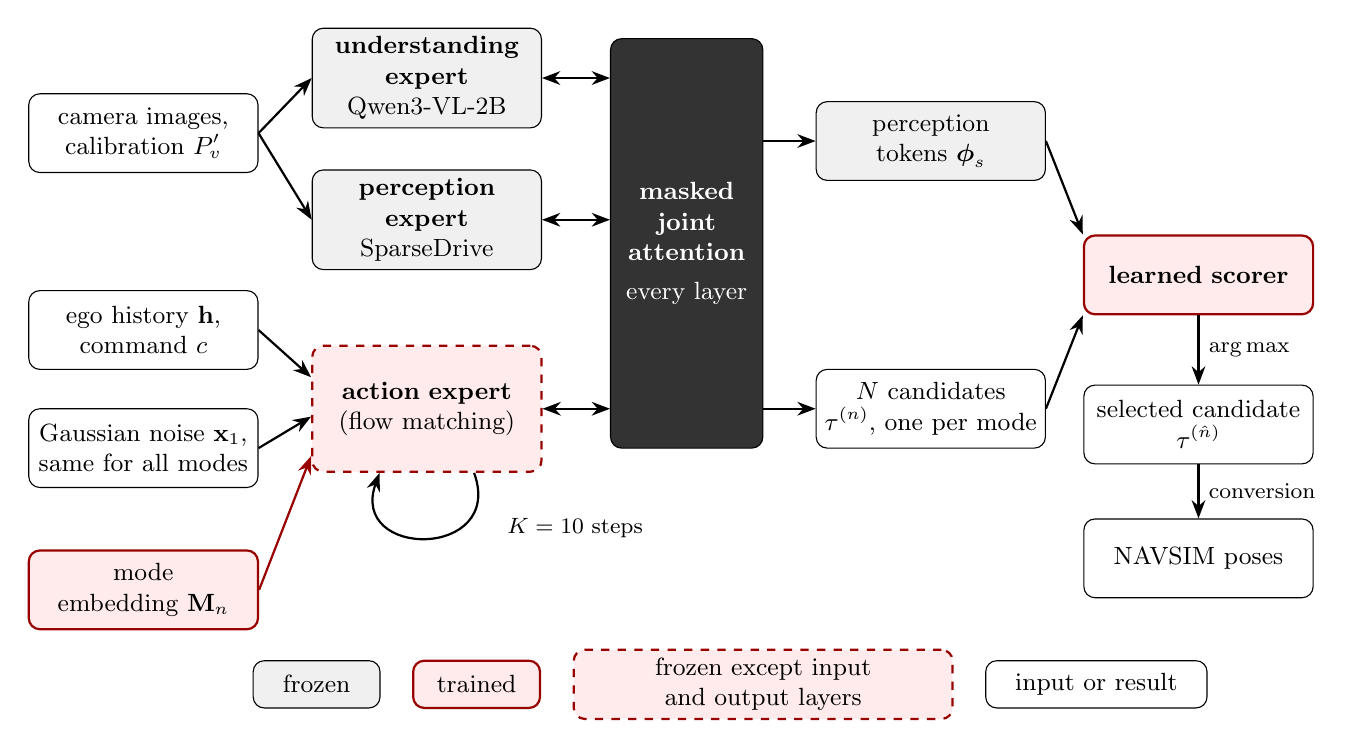
\begin{tikzpicture}[
  font=\small, >=Stealth,
  box/.style={draw,rounded corners,align=center,minimum height=1.0cm,text width=2.7cm,inner sep=3pt},
  frozen/.style={box,fill=gray!12},
  trained/.style={box,fill=red!8,draw=red!60!black,thick},
  part/.style={box,fill=red!8,draw=red!60!black,thick,dashed},
  plain/.style={box,fill=white},
  flow/.style={->,thick},
]
% inputs
\node[plain] (cam)   at (0,3.7)  {camera images,\\calibration $P'_v$};
\node[plain] (ego)   at (0,1.2)  {ego history $\mathbf h$,\\command $c$};
\node[plain] (noise) at (0,-0.3) {Gaussian noise $\mathbf x_1$,\\same for all modes};
\node[trained] (M)   at (0,-2.1) {mode\\embedding $\mathbf M_n$};
% experts
\node[frozen] (U) at (3.6,4.4) {\textbf{understanding}\\\textbf{expert}\\Qwen3-VL-2B};
\node[frozen] (P) at (3.6,2.6) {\textbf{perception}\\\textbf{expert}\\SparseDrive};
\node[part,minimum height=1.6cm] (A) at (3.6,0.2) {\textbf{action expert}\\(flow matching)};
\draw[flow] (cam.east) -- (U.west);
\draw[flow] (cam.east) -- (P.west);
\draw[flow] (ego.east) -- ([yshift=4mm]A.west);
\draw[flow] (noise.east) -- ([yshift=-1mm]A.west);
\draw[flow,red!60!black] (M.east) -- ([yshift=-6mm]A.west);
% denoising loop
\draw[->,thick] ([xshift=6mm]A.south) .. controls +(0.4,-1.1) and +(-0.4,-1.1) .. ([xshift=-6mm]A.south);
\node[font=\footnotesize,anchor=west] at ([xshift=9mm,yshift=-7mm]A.south) {$K=10$ steps};
% joint attention
\node[draw,rounded corners,fill=black!80,text=white,align=center,text width=1.7cm,
      minimum height=5.2cm] (J) at (6.9,2.3) {\textbf{masked}\\\textbf{joint}\\\textbf{attention}\\[3pt]every layer};
\draw[<->,thick] (U.east) -- (U.east -| J.west);
\draw[<->,thick] (P.east) -- (P.east -| J.west);
\draw[<->,thick] (A.east) -- (A.east -| J.west);
% outputs
\node[frozen] (phi)  at (10.0,3.6) {perception\\tokens $\boldsymbol\phi_s$};
\node[plain]  (traj) at (10.0,0.2) {$N$ candidates\\$\tau^{(n)}$, one per mode};
\draw[flow] (J.east |- phi) -- (phi.west);
\draw[flow] (J.east |- traj) -- (traj.west);
\node[trained] (sc)  at (13.4,1.9) {\textbf{learned scorer}};
\draw[flow] (phi.east) -- (sc.north west);
\draw[flow] (traj.east) -- (sc.south west);
\node[plain] (sel)  at (13.4,0.0) {selected candidate\\$\tau^{(\hat n)}$};
\node[plain] (conv) at (13.4,-1.7) {NAVSIM poses};
\draw[flow] (sc) -- node[right,font=\footnotesize]{$\arg\max$} (sel);
\draw[flow] (sel) -- node[right,font=\footnotesize]{conversion} (conv);
% legend
\node[frozen,text width=1.4cm,minimum height=0.6cm]  (l1) at (2.2,-3.3) {frozen};
\node[trained,text width=1.4cm,minimum height=0.6cm,right=0.4cm of l1] (l2) {trained};
\node[part,text width=4.6cm,minimum height=0.6cm,right=0.4cm of l2] (l3) {frozen except input and output layers};
\node[plain,text width=2.6cm,minimum height=0.6cm,right=0.4cm of l3] (l4) {input or result};
\end{tikzpicture}%
}
\caption[System overview]{\textbf{System overview.} The understanding and perception experts read
the camera images once per scene. The action expert turns Gaussian noise into a trajectory in
$K=10$ steps and is run once for each of the $N$ mode embeddings. The three experts exchange
information through masked joint attention. The learned scorer selects one candidate using the
perception tokens, and the selected candidate is converted to NAVSIM poses.}
\label{fig:framework}
\end{figure}


\section{Notation}
\label{sec:notation}
All coordinates are in the \emph{ego frame}, which is fixed to the vehicle, with $x$ pointing
forward and $y$ to the left. A \emph{pose} is a position with a heading. The inputs are
\begin{itemize}
  \item the images $I_v$ of $V=6$ cameras, $v=1,\dots,V$, resized as described in
  Section~\ref{sec:geometry};
  \item the ego history $\mathbf{h}\in\mathbb{R}^{T_h\times 2}$, the ego positions at the last
  $T_h=4$ frames in the current ego frame;
  \item the navigation command $c\in\{\textsf{left},\textsf{straight},\textsf{right}\}$.
  NAVSIM's command has a fourth value, \textsf{unknown}, which we map to \textsf{straight}.
\end{itemize}
The output is a trajectory $\tau=(\mathbf{p}_1,\dots,\mathbf{p}_T)$ of $T=6$ future positions
$\mathbf{p}_k\in\mathbb{R}^2$ at intervals of $\Delta t=\SI{0.5}{\second}$, a horizon of
\SI{3}{\second}. With $N$ modes, the planner outputs $N$ candidates $\tau^{(0)},\dots,\tau^{(N-1)}$.

\section{Camera adaptation}
\label{sec:geometry}
The perception expert places learned queries in 3D space and projects them into each camera
image to read image features. It therefore needs, for each camera, the matrix that maps a 3D
point to image coordinates. UniDriveVLA expresses 3D points in the frame of the vehicle's LiDAR
sensor, as in nuScenes. For camera $v$, let $R_v\in SO(3)$ and $\mathbf{t}_v\in\mathbb{R}^3$
be the rotation and translation from the LiDAR frame to the camera frame (the
\emph{extrinsics}), and $K_v\in\mathbb{R}^{3\times3}$ the camera's focal lengths and optical
centre (the \emph{intrinsics}). A point $\mathbf{X}$ in the LiDAR frame projects to image
coordinates $\mathbf{u}$ as
\begin{equation}
  \lambda\begin{bmatrix}\mathbf{u}\\1\end{bmatrix}
  = P_v\begin{bmatrix}\mathbf{X}\\1\end{bmatrix},\qquad
  P_v=K_v\,\big[\,R_v\mid\mathbf{t}_v\,\big]\in\mathbb{R}^{3\times4},
\end{equation}
where $\lambda$ is the depth of the point. NAVSIM provides the transform from each camera to
the LiDAR frame, $(R'_v,\mathbf{t}'_v)$; its inverse gives $R_v=R_v'^{\top}$ and
$\mathbf{t}_v=-R_v'^{\top}\mathbf{t}'_v$.

NAVSIM records eight cameras, and nuScenes six. We keep the six NAVSIM cameras whose positions
match the nuScenes cameras (front, front left, front right, back left, back right, back) and
drop the two additional side cameras. Each image is resized from
$(W_0,H_0)=(1920,1080)$ to the input size of UniDriveVLA, $(W,H)=(960,544)$. The intrinsics
are scaled accordingly,
\begin{equation}
  K'_v=S\,K_v,\qquad S=\operatorname{diag}\!\Big(\tfrac{W}{W_0},\ \tfrac{H}{H_0},\ 1\Big),
\end{equation}
and the model receives $P'_v=K'_v[R_v\mid\mathbf{t}_v]$. Figure~\ref{fig:inputadapt} shows these
steps.

\begin{figure}[t]
\centering
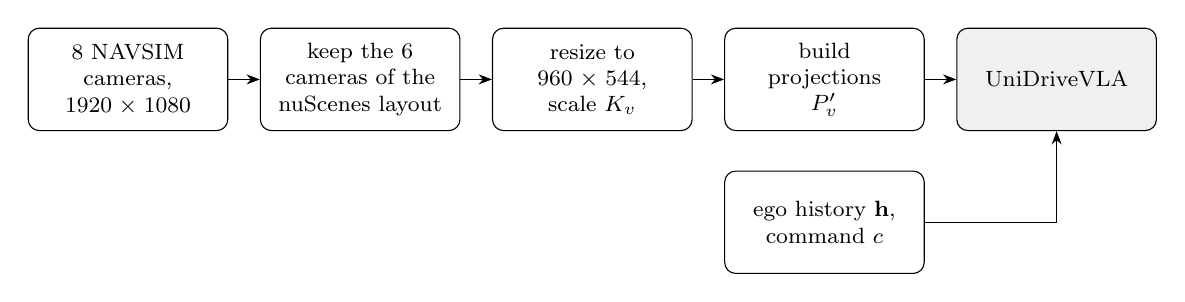
\begin{tikzpicture}[font=\small,>=Stealth,
  b/.style={draw,rounded corners,align=center,minimum height=1.3cm,text width=2.3cm,font=\footnotesize}]
  \node[b] (c8) {8 NAVSIM\\cameras,\\$1920\times1080$};
  \node[b,right=0.4cm of c8] (c6) {keep the 6\\cameras of the\\nuScenes layout};
  \node[b,right=0.4cm of c6] (rs) {resize to\\$960\times544$,\\scale $K_v$};
  \node[b,right=0.4cm of rs] (pr) {build\\projections\\$P'_v$};
  \node[b,fill=gray!12,right=0.4cm of pr] (in) {UniDriveVLA};
  \foreach \a/\bb in {c8/c6,c6/rs,rs/pr,pr/in}{\draw[->] (\a) -- (\bb);}
  \node[b,below=0.5cm of pr] (ex) {ego history $\mathbf h$,\\command $c$};
  \draw[->] (ex) -| (in);
\end{tikzpicture}
\caption[Camera adaptation]{\textbf{Camera adaptation.} Six of NAVSIM's eight cameras are kept and
resized, and the projection matrices are rebuilt for the new image size.}
\label{fig:inputadapt}
\end{figure}

\section{UniDriveVLA experts}
\label{sec:moe}
Each of UniDriveVLA's three experts \cite{unidrivevla} processes its own set of tokens, the
vectors a transformer operates on.

\paragraph{Understanding expert.} The understanding expert is the pretrained vision--language
model Qwen3-VL-2B \cite{qwen3vl}. It encodes the camera images and a text prompt into tokens
$F_\mathrm{u}$.

\paragraph{Perception expert.} The perception expert follows SparseDrive \cite{sparsedrive}.
It holds a fixed number of learned queries of two kinds: object queries, which detect other
road users, and map queries, which detect map elements such as lane boundaries. Each query is
updated with image features read through the projections $P'_v$ of
Section~\ref{sec:geometry}. Its output tokens are the perception tokens
$\boldsymbol{\phi}_s\in\mathbb{R}^{T_s\times256}$ of scene $s$.

\paragraph{Action expert.} The action expert generates the trajectory
(Section~\ref{sec:flow}). It processes two kinds of tokens. Two status tokens describe the ego
vehicle: one encodes the ego history $\mathbf{h}$, the other encodes the command $c$ together
with the ego vehicle's current motion state (10 values). During training the motion state is
taken from the recorded data. At inference the perception expert estimates it, as in the
released model; the ego state recorded by NAVSIM is not used. Six action tokens
$\boldsymbol{\alpha}_1,\dots,\boldsymbol{\alpha}_T$ represent the trajectory being generated,
one token per future position.

\paragraph{Masked joint attention.}
Each expert is a stack of transformer layers, and the three stacks have the same number of
layers. The experts do not only exchange their final outputs. In every layer, the tokens of all
three experts take part in one shared attention operation, while each expert keeps its own
weights. In attention, every token computes three vectors from its current representation: a
query, which describes what the token looks for; a key, which describes what the token
contains; and a value, the information the token passes on. For the tokens $F_g$ of expert
$g\in\{\mathrm{u},\mathrm{p},\mathrm{a}\}$ (understanding, perception, action) in one layer,
\begin{equation}
  Q_g=F_gW^Q_g,\qquad K_g=F_gW^K_g,\qquad V_g=F_gW^V_g ,
\end{equation}
where the weight matrices $W^Q_g$, $W^K_g$, and $W^V_g$ belong to expert $g$. The queries of
the three experts are stacked into one matrix $Q=[Q_\mathrm{u};Q_\mathrm{p};Q_\mathrm{a}]$,
likewise for $K$ and $V$. The attention output is
\begin{equation}
  Z=\operatorname{softmax}\!\Big(\tfrac{QK^\top}{\sqrt{d_k}}+M\Big)V ,
\end{equation}
where $d_k$ is the length of a key. Each row of $Z$ is a weighted sum of the values of all
tokens, with weights given by how well the token's query matches the other tokens' keys. The
mask $M$ decides which tokens a token may attend to. Its entry is $0$ if the token of the row
(the query) may attend to the token of the column (the key), and $-\infty$ otherwise, which sets the corresponding weight to
zero. Understanding tokens attend only to earlier understanding tokens. Perception tokens attend to
understanding and perception tokens. Action tokens attend to the tokens of all three experts
(Figure~\ref{fig:mask}).
Information therefore flows from the understanding and perception experts into the action
expert, while the action expert does not influence the other two. The rows of $Z$ that belong
to expert $g$ are that expert's attention output in this layer. The expert processes them
further with its own feed-forward layer and passes the result to its next layer.

% Attention mask of masked joint attention: which tokens (rows) may read which tokens (columns).
\begin{figure}[tb]
\centering
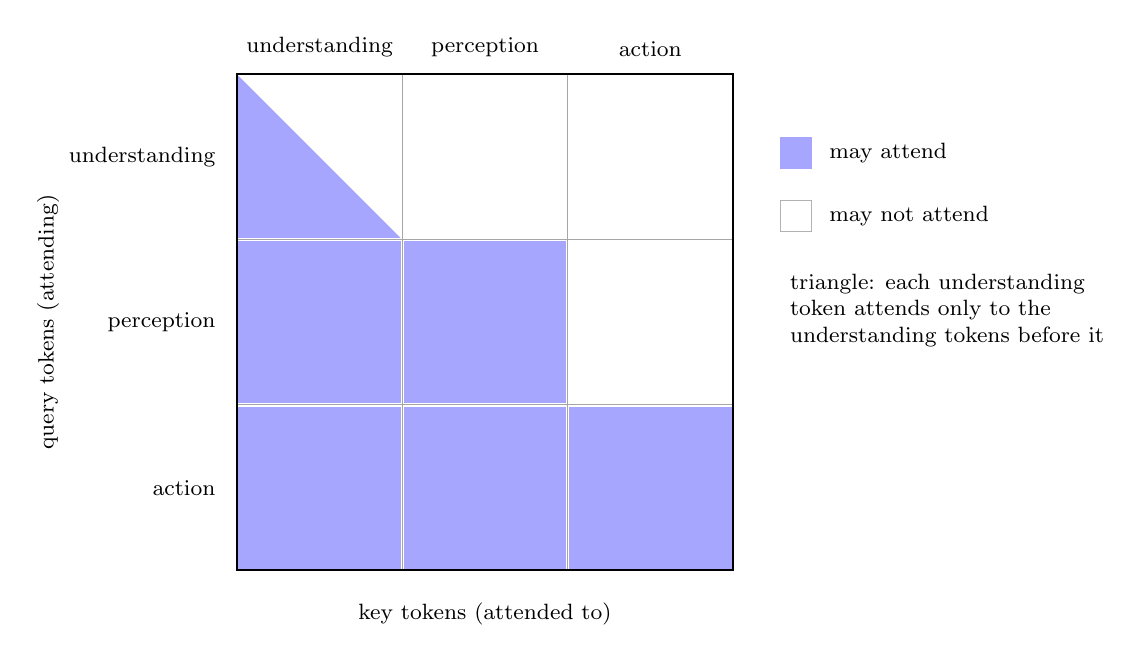
\begin{tikzpicture}[font=\small,>=Stealth]
  \def\s{2.1}
  % grid cells: rows (readers) top to bottom U,P,A ; columns (read) left to right U,P,A
  \foreach \r/\rl in {0/understanding,1/perception,2/action}{
    \node[anchor=east,font=\footnotesize] at (-0.15,{-(\r+0.5)*\s}) {\rl};
    \foreach \c in {0,1,2}{
      \draw[gray!60] ({\c*\s},{-\r*\s}) rectangle ({(\c+1)*\s},{-(\r+1)*\s});
    }
  }
  \foreach \c/\cl in {0/understanding,1/perception,2/action}
    \node[anchor=south,font=\footnotesize] at ({(\c+0.5)*\s},0.1) {\cl};
  % allowed blocks
  \fill[blue!35] (0,0) -- (0,-\s) -- (\s,-\s) -- cycle;             % U reads earlier U (causal)
  \fill[blue!35] (0,-\s) rectangle (2*\s,-2*\s);                    % P reads U, P
  \fill[blue!35] (0,-2*\s) rectangle (3*\s,-3*\s);                  % A reads U, P, A
  \foreach \i in {1,2}{\draw[white,very thick] ({\i*\s},0) -- ({\i*\s},-3*\s); \draw[white,very thick] (0,{-\i*\s}) -- (3*\s,{-\i*\s});}
  \foreach \i in {1,2}{\draw[gray!70] ({\i*\s},0) -- ({\i*\s},-3*\s); \draw[gray!70] (0,{-\i*\s}) -- (3*\s,{-\i*\s});}
  \draw[thick] (0,0) rectangle (3*\s,-3*\s);
  \node[font=\footnotesize,align=center] at ({1.5*\s},{-3*\s-0.55}) {key tokens (attended to)};
  \node[font=\footnotesize,rotate=90,align=center] at (-2.4,{-1.5*\s}) {query tokens (attending)};
  % legend
  \fill[blue!35] (6.9,-1.2) rectangle (7.3,-0.8); \node[anchor=west,font=\footnotesize] at (7.4,-1.0) {may attend};
  \draw[gray!60] (6.9,-2.0) rectangle (7.3,-1.6); \node[anchor=west,font=\footnotesize] at (7.4,-1.8) {may not attend};
  \node[anchor=west,font=\footnotesize,align=left] at (6.9,-3.0) {triangle: each understanding\\token attends only to the\\understanding tokens before it};
\end{tikzpicture}
\caption[Attention mask of masked joint attention]{\textbf{Attention mask of masked joint
attention}, applied in every layer. Each row shows which tokens the queries of one expert may
attend to. The action expert attends to all tokens; no expert attends to the action tokens.}
\label{fig:mask}
\end{figure}


\section{Trajectory generation with flow matching}
\label{sec:flow}
The action expert generates trajectories with flow matching \cite{flowmatching}. Let
$\mathbf{a}\in\mathbb{R}^{T\times2}$ be the recorded trajectory, written as displacements
between consecutive positions and standardised with the mean and standard deviation of the
training set. For noise $\boldsymbol{\epsilon}\sim\mathcal{N}(0,I)$ and time
$t\sim\mathcal{U}(0,1)$, flow matching defines the point
\begin{equation}
  \mathbf{x}_t=(1-t)\,\mathbf{a}+t\,\boldsymbol{\epsilon}
\end{equation}
on a straight path from $\mathbf{a}$ ($t=0$) to $\boldsymbol{\epsilon}$ ($t=1$), whose
velocity is $\mathbf{u}=\boldsymbol{\epsilon}-\mathbf{a}$. Each action token is computed from
the corresponding row of $\mathbf{x}_t$ and an embedding of $t$. The action expert's output
layer maps the action tokens to a predicted velocity $v_\theta(\mathbf{x}_t,t,s)$. Here $s$
stands for the scene: the understanding and perception tokens that the action tokens attend to.

The training loss has two terms. The first compares the predicted velocity with $\mathbf{u}$.
The second compares positions in metres. From the predicted velocity $v=v_\theta(\mathbf{x}_t,t,s)$,
the recorded trajectory is estimated as $\hat{\mathbf{a}}=\mathbf{x}_t-t\,v$. Let
$\mathrm{P}(\cdot)$ convert standardised displacements back to metres and add them up into
positions. The loss for one sample is
\begin{equation}
  \ell(v)=w(t)\,\big\lVert v-\mathbf{u}\big\rVert^2
  +\beta\,\big\lVert \mathrm{P}(\hat{\mathbf{a}})-\mathrm{P}(\mathbf{a})\big\rVert^2,
  \qquad \beta=0.5,
  \label{eq:fmloss}
\end{equation}
and $\mathcal{L}_{\mathrm{fm}}$ is its mean over the training samples. In the second term, the
gradient of each position passes only through the last three displacements added to it. This
prevents large gradients through the cumulative sum. The weight
\begin{equation}
  w(t)=\frac{\min\{\mathrm{SNR}(t),\gamma\}}{\mathrm{SNR}(t)},\qquad
  \mathrm{SNR}(t)=\Big(\frac{1-t}{t}\Big)^2,\qquad \gamma=5,
\end{equation}
reduces the first term for small $t$, where the task is easiest \cite{minsnr}.

To generate a trajectory, the action expert starts from $\mathbf{x}_1=\boldsymbol{\epsilon}$
and takes $K=10$ Euler steps of size $\delta=1/K$ towards $t=0$,
\begin{equation}
  \mathbf{x}_{t-\delta}=\mathbf{x}_t-\delta\,v_\theta(\mathbf{x}_t,t,s) .
\end{equation}
The result $\mathbf{x}_0$ is converted back to metres and accumulated into the positions
$\tau$. The only random input is $\boldsymbol{\epsilon}$. Trained on one recorded trajectory
per scene, the released action expert returns nearly the same trajectory for different
$\boldsymbol{\epsilon}$ (Section~\ref{sec:diversity}). Figure~\ref{fig:flow} shows the
generation.

\begin{figure}[t]
\centering
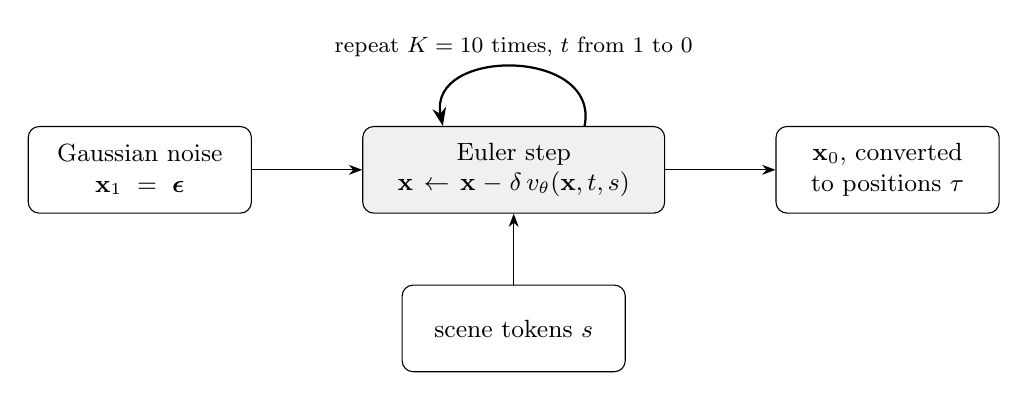
\begin{tikzpicture}[font=\small,>=Stealth,
  b/.style={draw,rounded corners,align=center,minimum height=1.1cm,text width=2.6cm}]
  \node[b] (n) {Gaussian noise\\$\mathbf{x}_1=\boldsymbol\epsilon$};
  \node[b,fill=gray!12,text width=3.6cm,right=1.4cm of n] (v)
       {Euler step\\$\mathbf{x}\leftarrow\mathbf{x}-\delta\,v_\theta(\mathbf{x},t,s)$};
  \node[b,right=1.4cm of v] (o) {$\mathbf{x}_0$, converted\\to positions $\tau$};
  \draw[->] (n) -- (v);
  \draw[->] (v) -- (o);
  \draw[->,thick] ([xshift=9mm]v.north) .. controls +(0.2,1.0) and +(-0.2,1.0) .. ([xshift=-9mm]v.north)
     node[pos=0.5,above,font=\footnotesize]{repeat $K=10$ times, $t$ from 1 to 0};
  \node[b,below=0.9cm of v] (c) {scene tokens $s$};
  \draw[->] (c) -- (v);
\end{tikzpicture}
\caption[Trajectory generation with flow matching]{\textbf{Trajectory generation with flow
matching.} Starting from Gaussian noise, the action expert applies $K=10$ Euler steps with the
predicted velocity $v_\theta$ to obtain a trajectory.}
\label{fig:flow}
\end{figure}

\section{Mode embeddings}
\label{sec:modes}
To obtain $N$ different candidates, we add a table of $N$ learned vectors
$\mathbf{M}\in\mathbb{R}^{N\times d}$, where $d=1024$ is the width of the action expert. Mode
$n$ adds row $\mathbf{M}_n$ to every action token before the first layer,
\begin{equation}
  \boldsymbol{\alpha}^{(n)}_k=\boldsymbol{\alpha}_k+\mathbf{M}_n,\qquad k=1,\dots,T,\quad
  n=0,\dots,N-1.
\end{equation}
The predicted velocity then depends on the mode, $v_\theta(\mathbf{x}_t,t,s,n)$, and the same
scene and noise give a different trajectory $\tau^{(n)}$ for each mode. This plays the role of
DrivoR's learned trajectory queries \cite{drivor}. We use $N=8$; the table has
$N\cdot d=\num{8192}$ parameters. Mode $n=0$ is the \emph{default mode}, the candidate the
planner returns without a scorer.

\section{Relaxed winner-takes-all training}
\label{sec:wta}
If all modes were trained towards the same recorded trajectory, they would become identical.
Winner-takes-all training \cite{mcl} avoids this by updating, for each scene, only the mode
with the lowest loss. We use its relaxed form \cite{rupprecht}: the mode with the lowest loss
receives most of the update, and the other modes receive a small share
(Figure~\ref{fig:wta}). The loss is the flow-matching loss of Equation~\eqref{eq:fmloss}.
It measures how far the velocity and the positions predicted by a mode are from those of the
recorded trajectory, so the winner is the mode that best reproduces the human driver's
trajectory. No driving score is used in this training; EPDMS is used only by the scorer
(Section~\ref{sec:selection}). For a batch of $B$ scenes, we draw one $(\boldsymbol{\epsilon}_i,t_i)$
per scene $i$, shared by all modes, and compute the loss of each mode with
Equation~\eqref{eq:fmloss},
\begin{equation}
  \ell_{i,n}=\ell\big(v_\theta(\mathbf{x}_{t_i},t_i,s_i,n)\big) .
\end{equation}
The training loss is
\begin{equation}
  \mathcal{L}_{\mathrm{wta}}=\frac{1}{B}\sum_{i=1}^{B}\Big[(1-\eta)\min_{n}\ell_{i,n}
  +\frac{\eta}{N}\sum_{n=0}^{N-1}\ell_{i,n}\Big],
\end{equation}
with $\eta=0.05$. The first term updates only the winning mode, since the derivative of
$\min_n\ell_{i,n}$ with respect to $\ell_{i,m}$ is $1$ for the winning mode and $0$ for the
others. The modes thus specialise on different scenes. The second term gives every mode a small
gradient, so that a mode that never wins is still trained.

% One training step of the mode embeddings (relaxed winner-takes-all).
\begin{figure}[tb]
\centering
\resizebox{\linewidth}{!}{%
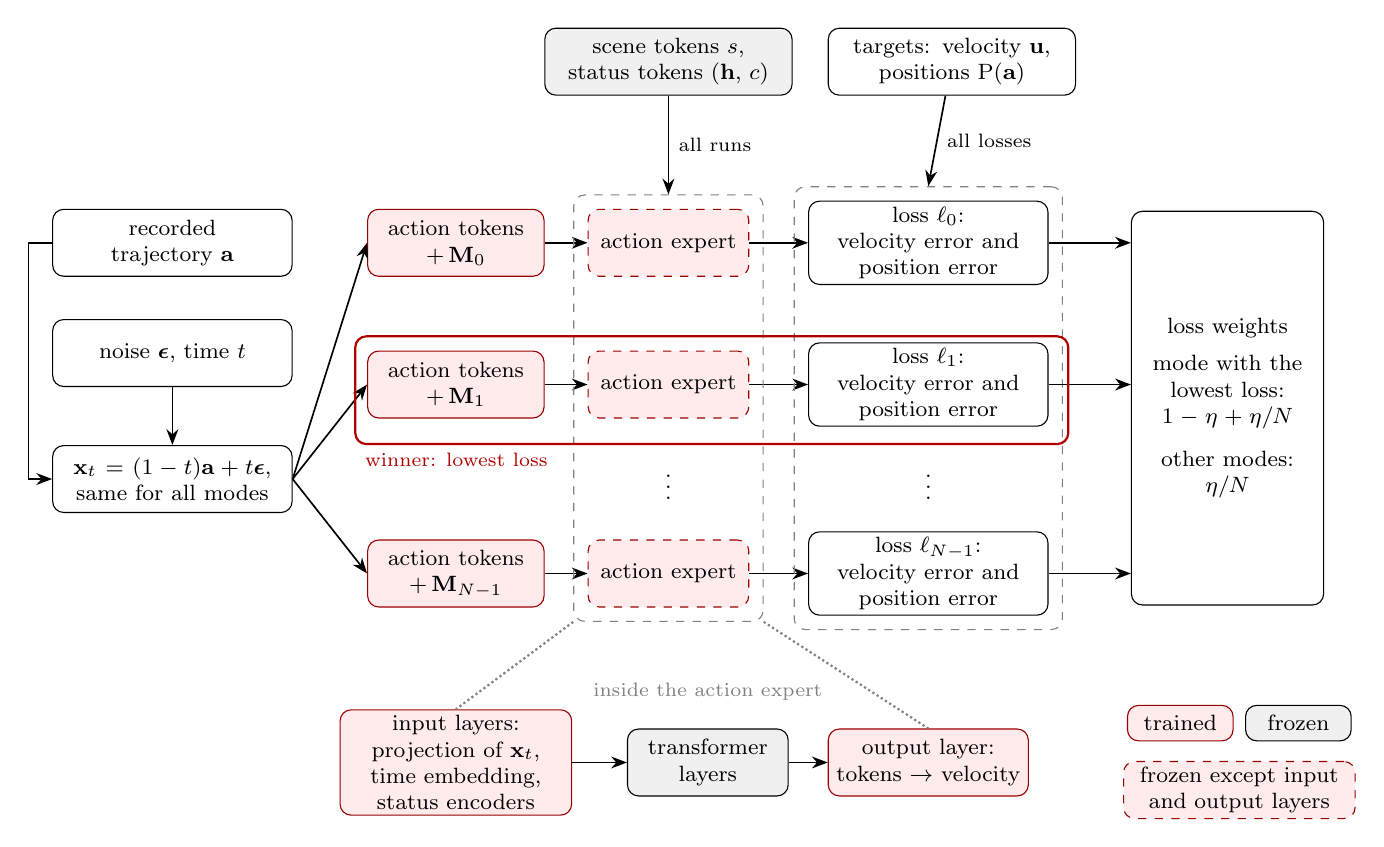
\begin{tikzpicture}[
  font=\footnotesize, >=Stealth,
  box/.style={draw,rounded corners,align=center,minimum height=0.85cm,inner sep=2pt},
  trn/.style={box,fill=red!8,draw=red!60!black},
  frz/.style={box,fill=gray!12},
  prt/.style={box,fill=red!8,draw=red!60!black,dashed},
  pln/.style={box,fill=white},
  flow/.style={->,semithick},
]
% shared inputs
\node[pln,text width=2.9cm] (a)  at (0,-1.6) {recorded\\trajectory $\mathbf a$};
\node[pln,text width=2.9cm] (et) at (0,-3.0) {noise $\boldsymbol\epsilon$, time $t$};
\node[pln,text width=2.9cm] (xt) at (0,-4.6) {$\mathbf x_t=(1-t)\mathbf a+t\boldsymbol\epsilon$,\\same for all modes};
\draw[flow] (et) -- (xt);
\draw[flow] (a.west) -- ++(-0.3,0) |- (xt.west);
% mode rows
\foreach \n/\lab/\y in {0/0/-1.6, 1/1/-3.4, 2/N-1/-5.8}{
  \node[trn,text width=2.1cm] (in\n) at (3.6,\y) {action tokens\\$+\,\mathbf M_{\lab}$};
  \node[prt,text width=1.9cm] (ae\n) at (6.3,\y) {action expert};
  \node[pln,text width=2.9cm] (l\n)  at (9.6,\y) {loss $\ell_{\lab}$:\\velocity error and\\position error};
  \draw[flow] (xt.east) -- (in\n.west);
  \draw[flow] (in\n) -- (ae\n);
  \draw[flow] (ae\n) -- (l\n);
}
\node at (6.3,-4.6) {$\vdots$};
\node at (9.6,-4.6) {$\vdots$};
% column groups with their shared inputs
\node[draw,dashed,gray,rounded corners,fit=(ae0)(ae2),inner sep=5pt] (gA) {};
\node[draw,dashed,gray,rounded corners,fit=(l0)(l2),inner sep=5pt] (gL) {};
\node[frz,text width=3.0cm] (sc) at (6.3,0.7) {scene tokens $s$,\\status tokens ($\mathbf h$, $c$)};
\node[pln,text width=3.0cm] (tg) at (9.9,0.7) {targets: velocity $\mathbf u$,\\positions $\mathrm P(\mathbf a)$};
\draw[flow] (sc) -- node[right,font=\scriptsize]{all runs} (gA.north);
\draw[flow] (tg) -- node[right,font=\scriptsize]{all losses} (gL.north);
% loss weights
\node[pln,text width=2.3cm,minimum height=5.0cm] (mn) at (13.4,-3.7)
  {loss weights\\[4pt]mode with the\\lowest loss:\\$1-\eta+\eta/N$\\[6pt]other modes:\\$\eta/N$};
\foreach \n in {0,1,2}{\draw[flow] (l\n.east) -- (l\n.east -| mn.west);}
% winner frame around row 1
\draw[red!70!black,thick,rounded corners] ($(in1.north west)+(-0.15,0.18)$) rectangle ($(l1.south east)+(0.25,-0.22)$);
\node[font=\scriptsize,text=red!70!black,anchor=north west] at ($(in1.south west)+(-0.15,-0.32)$) {winner: lowest loss};
% inside the action expert
\node[trn,text width=2.8cm] (d1) at (3.6,-8.2) {input layers: projection of $\mathbf x_t$, time embedding, status encoders};
\node[frz,text width=1.9cm] (d2) at (6.8,-8.2) {transformer\\layers};
\node[trn,text width=2.4cm] (d3) at (9.6,-8.2) {output layer:\\tokens $\to$ velocity};
\draw[flow] (d1) -- (d2);
\draw[flow] (d2) -- (d3);
\draw[gray,densely dotted,thick] (gA.south west) -- (d1.north);
\draw[gray,densely dotted,thick] (gA.south east) -- (d3.north);
\node[font=\scriptsize,text=gray] at (6.8,-7.3) {inside the action expert};
% legend
\node[trn,text width=1.2cm,minimum height=0.45cm] (k1) at (12.8,-7.7) {trained};
\node[frz,text width=1.2cm,minimum height=0.45cm] (k2) at (14.3,-7.7) {frozen};
\node[prt,text width=2.8cm,minimum height=0.45cm] (k3) at (13.55,-8.55) {frozen except input and output layers};
\end{tikzpicture}%
}
\caption[Training of the mode embeddings]{\textbf{Training of the mode embeddings.} For one
recorded scene, the same noisy trajectory $\mathbf x_t$ is passed through the action expert once
per mode, each time with a different mode embedding $\mathbf M_n$ added to the action tokens.
Each run predicts a velocity, and its loss $\ell_n$ combines the error of this velocity and the
error of the resulting positions (Equation~\eqref{eq:fmloss}). The mode with the lowest loss
receives most of the update; the other modes receive a small share, set by $\eta=0.05$.}
\label{fig:wta}
\end{figure}


The trained parameters are
\begin{itemize}
  \item the mode table $\mathbf{M}$;
  \item the input layers of the action expert: the projection of $\mathbf{x}_t$ into the action
  tokens, the embedding of the time $t$, and the encoders that compute the status tokens from
  the ego history and the command;
  \item the output layer of the action expert, which maps the action tokens to the velocity.
\end{itemize}
Together these have about \num{5.3} million parameters. All other parameters of UniDriveVLA are frozen
(Table~\ref{tab:stages}). Training uses the nuScenes training split; Table~\ref{tab:hparams}
lists the settings.

\begin{table}[ht]
\centering
\caption[Trained and frozen components]{Trained and frozen components.}
\label{tab:stages}
\begin{tabularx}{\linewidth}{@{}>{\raggedright\arraybackslash}X >{\raggedright\arraybackslash}X l r@{}}
\toprule
Component & Training data & Status & Parameters \\
\midrule
Understanding expert (Qwen3-VL-2B), perception expert, and transformer layers of the action expert & images and text, nuScenes & frozen & $\approx$2.7\,B \\
Action expert, input and output layers, and mode table & nuScenes & trained & $\approx$5.3\,M \\
Learned scorer & navhard, five-fold cross-validation & trained & $\approx$0.13\,M \\
\bottomrule
\end{tabularx}
\end{table}



\section{Conversion to NAVSIM}
\label{sec:output}
UniDriveVLA outputs six positions over \SI{3}{\second}, whereas NAVSIM expects eight poses
$(x,y,\theta)$ over \SI{4}{\second}. The conversion has three steps (Figure~\ref{fig:outconv}).

\paragraph{Axes.} UniDriveVLA stores each position as (lateral, forward), $(\ell_k,f_k)$.
NAVSIM uses $x$ forward and $y$ left, so
\begin{equation}
  x_k=f_k,\qquad y_k=\zeta\,\ell_k,\qquad \zeta=-1 .
\end{equation}
We verified the sign $\zeta$ on navhard: converting NAVSIM's recorded future positions into
the model's convention and back reproduces them only with $\zeta=-1$. The wrong sign would
mirror every turn.

\paragraph{Horizon.} UniDriveVLA predicts $T=6$ positions (\SI{3}{\second}), NAVSIM expects
$T'=8$ (\SI{4}{\second}). The two missing positions continue the trajectory at the speed and
direction of its last step: each adds the last displacement $\mathbf{p}_T-\mathbf{p}_{T-1}$
once more,
\begin{equation}
  \mathbf{p}_k=\mathbf{p}_T+(k-T)\,(\mathbf{p}_T-\mathbf{p}_{T-1}),\qquad k=7,8 .
\end{equation}
This extension only makes the trajectory compatible with NAVSIM v2; in a turn it continues
straight. Section~\ref{sec:limits} discusses its possible effect.

\paragraph{Heading.} Each pose receives the direction of the displacement that leads to it,
\begin{equation}
  \theta_k=\operatorname{atan2}\big(y_k-y_{k-1},\ x_k-x_{k-1}\big),\qquad
  k=1,\dots,T',\quad \mathbf{p}_0=(0,0).
\end{equation}

% Conversion to NAVSIM, drawn on an example left turn: model frame (lateral, forward) on the
% left; NAVSIM frame (x forward, y left) with the two extended positions and headings on the right.
\begin{figure}[tb]
\centering
\resizebox{\linewidth}{!}{%
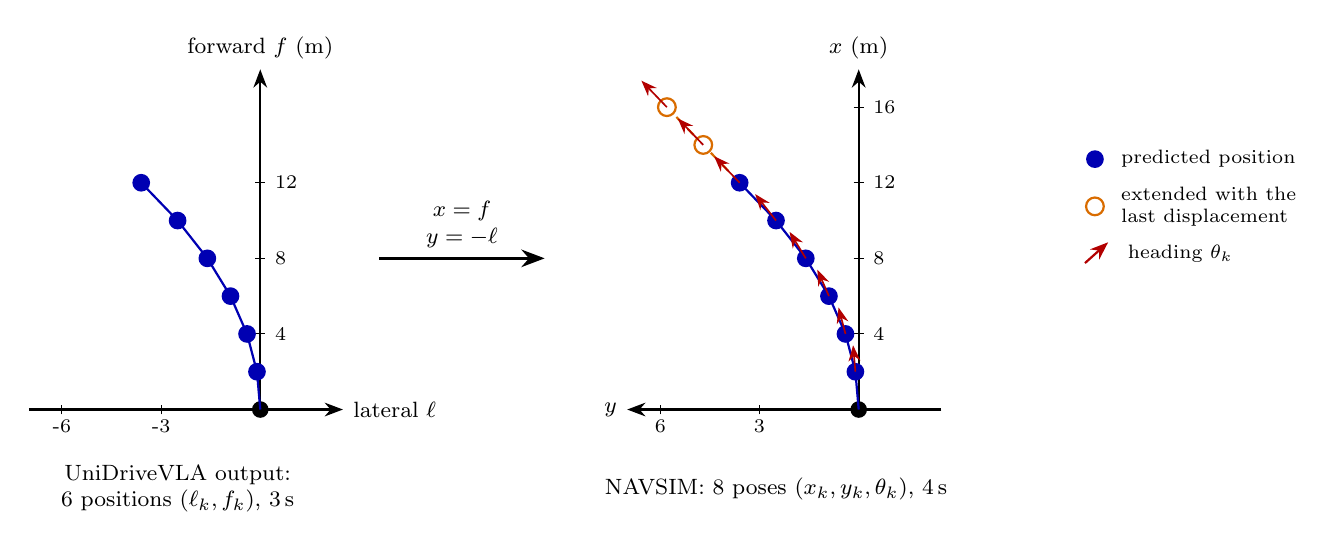
\begin{tikzpicture}[font=\small,>=Stealth,x=0.42cm,y=0.24cm]
% ---------------- left panel: UniDriveVLA output ----------------
\begin{scope}
  \draw[->,thick] (0,0) -- (0,18) node[above,font=\footnotesize] {forward $f$ (m)};
  \draw[->,thick] (-7,0) -- (2.5,0) node[right,font=\footnotesize] {lateral $\ell$};
  \foreach \yy in {4,8,12} \draw (-0.15,\yy) -- (0.15,\yy) node[right,font=\scriptsize] {\yy};
  \foreach \xx in {-6,-3} \draw (\xx,-0.25) -- (\xx,0.25) node[below=2pt,font=\scriptsize] {\xx};
  \fill[black] (0,0) circle (3pt);
  \draw[blue!70!black,thick] (0,0) -- (-0.1,2) -- (-0.4,4) -- (-0.9,6) -- (-1.6,8) -- (-2.5,10) -- (-3.6,12);
  \foreach \p in {(-0.1,2),(-0.4,4),(-0.9,6),(-1.6,8),(-2.5,10),(-3.6,12)}
    \fill[blue!70!black] \p circle (3.2pt);
  \node[font=\footnotesize,align=center] at (-2.5,-4.2) {UniDriveVLA output:\\6 positions $(\ell_k,f_k)$, \SI{3}{\second}};
\end{scope}
% arrow between panels
\draw[->,very thick] (3.6,8) -- node[above,font=\footnotesize,align=center]{$x=f$\\$y=-\ell$} (8.6,8);
% ---------------- right panel: NAVSIM poses ----------------
\begin{scope}[xshift=7.6cm]
  \draw[->,thick] (0,0) -- (0,18) node[above,font=\footnotesize] {$x$ (m)};
  \draw[->,thick] (2.5,0) -- (-7,0) node[left,font=\footnotesize] {$y$};
  \foreach \yy in {4,8,12,16} \draw (-0.15,\yy) -- (0.15,\yy) node[right,font=\scriptsize] {\yy};
  \foreach \xx/\lab in {-3/3,-6/6} \draw (\xx,-0.25) -- (\xx,0.25) node[below=2pt,font=\scriptsize] {\lab};
  \fill[black] (0,0) circle (3pt);
  \draw[blue!70!black,thick] (0,0) -- (-0.1,2) -- (-0.4,4) -- (-0.9,6) -- (-1.6,8) -- (-2.5,10) -- (-3.6,12);
  \draw[orange!85!black,thick,dashed] (-3.6,12) -- (-4.7,14) -- (-5.8,16);
  \foreach \p in {(-0.1,2),(-0.4,4),(-0.9,6),(-1.6,8),(-2.5,10),(-3.6,12)}
    \fill[blue!70!black] \p circle (3.2pt);
  \foreach \p in {(-4.7,14),(-5.8,16)}
    \draw[orange!85!black,fill=white,thick] \p circle (3.2pt);
  % headings: direction of the displacement leading to each pose
  \coordinate (q0) at (0,0);    \coordinate (q1) at (-0.1,2); \coordinate (q2) at (-0.4,4);
  \coordinate (q3) at (-0.9,6); \coordinate (q4) at (-1.6,8); \coordinate (q5) at (-2.5,10);
  \coordinate (q6) at (-3.6,12);\coordinate (q7) at (-4.7,14);\coordinate (q8) at (-5.8,16);
  \foreach \k [evaluate=\k as \km using int(\k-1)] in {1,...,8}
    \draw[->,red!70!black,semithick] (q\k) -- ($(q\k)+0.7*(q\k)-0.7*(q\km)$);
  \node[font=\footnotesize,align=center] at (-2.5,-4.2) {NAVSIM: 8 poses $(x_k,y_k,\theta_k)$, \SI{4}{\second}};
\end{scope}
% legend
\begin{scope}[xshift=10.6cm,yshift=0.3cm]
  \fill[blue!70!black] (0,12) circle (3.2pt); \node[anchor=west,font=\scriptsize] at (0.5,12) {predicted position};
  \draw[orange!85!black,fill=white,thick] (0,9.5) circle (3.2pt); \node[anchor=west,font=\scriptsize,align=left] at (0.5,9.5) {extended with the\\last displacement};
  \draw[->,red!70!black,thick] (-0.3,6.5) -- (0.4,7.6); \node[anchor=west,font=\scriptsize,align=left] at (0.7,7) {heading $\theta_k$};
\end{scope}
\end{tikzpicture}%
}
\caption[Conversion to NAVSIM]{\textbf{Conversion to NAVSIM}, shown for a left turn. The model
measures the lateral coordinate to the right, NAVSIM measures $y$ to the left; both panels
show the same path. The six predicted positions are extended to eight by repeating the last
displacement, and each pose receives the heading of the displacement that leads to it.}
\label{fig:outconv}
\end{figure}


\section{EPDMS}
\label{sec:epdms}
The scorer predicts the terms of EPDMS, the metric of NAVSIM v2 \cite{pseudosim}, so we state
its exact form. For a trajectory $\tau$ in a scene $s$, NAVSIM v2 computes nine terms in
$[0,1]$. Four are penalty terms:
\begin{itemize}
  \item no at-fault collision (NC): the ego vehicle does not cause a collision;
  \item drivable-area compliance (DAC): the ego vehicle stays on the drivable area;
  \item driving-direction compliance (DDC): the ego vehicle does not drive against the
  direction of its lane outside intersections;
  \item traffic-light compliance (TLC): the ego vehicle does not pass a red light.
\end{itemize}
Five are quality terms:
\begin{itemize}
  \item ego progress (EP): how far the ego vehicle advances along its route;
  \item time to collision (TTC): the ego vehicle keeps a safe time gap to other road users;
  \item history comfort (HC): acceleration and jerk stay within comfort limits when the
  trajectory is joined to the vehicle's recorded motion before it;
  \item lane keeping (LK): the ego vehicle stays close to the centre of its lane;
  \item extended comfort (EC): the trajectory is consistent with the one planned in the
  previous frame, without jumps in acceleration or jerk.
\end{itemize}
NAVSIM v2 combines the nine terms of one trajectory in one scene into a single score. We call
this score the \emph{stage score}, because it is computed separately for every scene of both
stages before EPDMS combines them:
\begin{equation}
  m(\tau,s)=\Big(\prod_{c\in\mathcal{P}} c\Big)\cdot\frac{\sum_{j\in\mathcal{Q}} w_j\,q_j}
  {\sum_{j\in\mathcal{Q}} w_j},
  \label{eq:epdms}
\end{equation}
where $\mathcal{P}$ is the set of penalty terms, $\mathcal{Q}$ the set of quality terms, and
the weights are $(w_{\mathrm{EP}},w_{\mathrm{TTC}},w_{\mathrm{HC}},w_{\mathrm{LK}},w_{\mathrm{EC}})
=(5,5,2,2,2)$. If any penalty term is zero, the stage score is zero.

NAVSIM v2 evaluates each scene $s$ in two stages \cite{pseudosim} (Figure~\ref{fig:twostage}).
In the first stage, the planner predicts a trajectory $\tau$ from the recorded scene. This
trajectory receives the stage score $m(\tau,s)$ and ends at the position $\hat{x}$.

The second stage tests the planner four seconds later, from positions near the ones it may
reach. NAVSIM renders $J$ new scenes $s_j$ in which the ego vehicle starts at positions $x_j$
around the recorded position of the human driver after four seconds. The planner predicts a new
trajectory $\tau_j$ in each of them, which receives the stage score $m(\tau_j,s_j)$. The planner's own
first-stage trajectory ends at $\hat{x}$, not necessarily at the human driver's position, so
each stage score of the second stage is weighted by how close its start position $x_j$ is to
$\hat{x}$.

EPDMS multiplies the first-stage score with the weighted mean of the second-stage scores:
\begin{equation}
  \mathrm{EPDMS}(s)=m(\tau,s)\cdot\frac{\sum_{j=1}^{J}\omega_j\,m(\tau_j,s_j)}
  {\sum_{j=1}^{J}\omega_j},\qquad
  \omega_j=\exp\!\Big(-\frac{\lVert x_j-\hat{x}\rVert^2}{2\sigma^2}\Big),
\end{equation}
where $\sigma$ is a fixed constant. The reported EPDMS is the mean of $\mathrm{EPDMS}(s)$ over
all scenes, multiplied by 100.

% NAVSIM v2 two-stage scoring, bird's-eye sketches (x forward to the right).
\begin{figure}[tb]
\centering
\resizebox{\linewidth}{!}{%
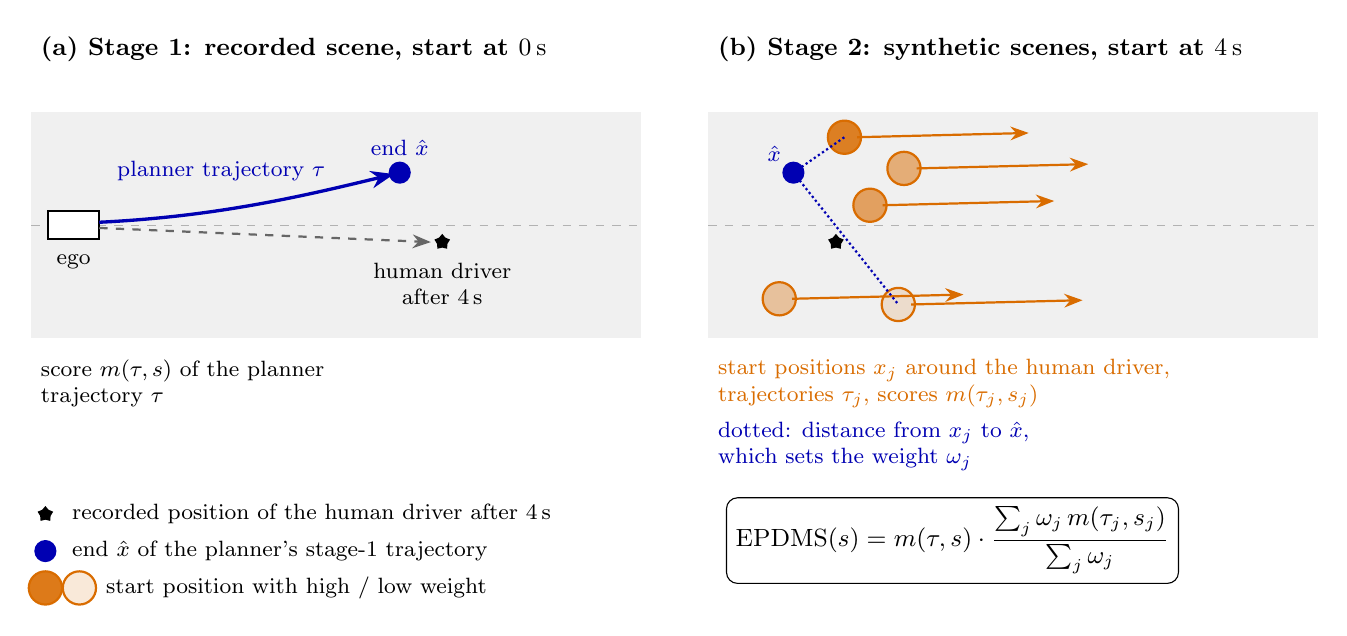
\begin{tikzpicture}[font=\footnotesize,>=Stealth,x=0.36cm,y=0.36cm]
  % ---------------- (a) stage 1 ----------------
  \begin{scope}
    \node[anchor=west,font=\small\bfseries] at (-1.5,6.2) {(a) Stage 1: recorded scene, start at \SI{0}{\second}};
    \fill[gray!12] (-1.5,-4) rectangle (20,4);
    \draw[gray!60,dashed] (-1.5,0) -- (20,0);
    \draw[fill=white,thick] (-0.9,-0.5) rectangle (0.9,0.5);
    \node[anchor=north] at (0,-0.7) {ego};
    % recorded human future
    \draw[black!60,thick,dashed,->] (0.9,-0.1) -- (12.6,-0.6);
    \node[star,star points=5,fill=black,inner sep=1.4pt] at (13,-0.6) {};
    \node[anchor=north,align=center] at (13,-1.0) {human driver\\after \SI{4}{\second}};
    % planner trajectory
    \draw[blue!70!black,very thick,->] (0.9,0.1) .. controls (5,0.3) and (8,1.0) .. (11.3,1.8);
    \fill[blue!70!black] (11.5,1.85) circle (4pt);
    \node[blue!70!black,anchor=south] at (11.5,2.1) {end $\hat x$};
    \node[blue!70!black,anchor=south] at (5.2,1.2) {planner trajectory $\tau$};
    \node[anchor=north west,align=left] at (-1.5,-4.4) {score $m(\tau,s)$ of the planner\\trajectory $\tau$};
  \end{scope}
  % ---------------- (b) stage 2 ----------------
  \begin{scope}[xshift=8.6cm]
    \node[anchor=west,font=\small\bfseries] at (-1.5,6.2) {(b) Stage 2: synthetic scenes, start at \SI{4}{\second}};
    \fill[gray!12] (-1.5,-4) rectangle (20,4);
    \draw[gray!60,dashed] (-1.5,0) -- (20,0);
    % reference points carried over
    \node[star,star points=5,fill=black,inner sep=1.4pt] at (3,-0.6) {};
    \fill[blue!70!black] (1.5,1.85) circle (4pt);
    \node[blue!70!black,anchor=south east] at (1.4,1.9) {$\hat x$};
    % synthetic start positions around the human position
    \foreach \px/\py/\op in {3.3/3.1/0.85, 1.0/-2.6/0.35, 5.2/-2.8/0.15, 5.4/2.0/0.5, 4.2/0.7/0.6}{
      \draw[orange!85!black,fill=orange!85!black,fill opacity=\op,thick] (\px,\py) circle (6pt);
      \draw[orange!85!black,thick,->] (\px+0.45,\py) -- (\px+6.5,\py+0.15);
    }
    \draw[blue!70!black,densely dotted,thick] (1.5,1.85) -- (3.3,3.1);
    \draw[blue!70!black,densely dotted,thick] (1.5,1.85) -- (5.2,-2.8);
    \node[orange!85!black,anchor=north west,align=left] at (-1.5,-4.4) {start positions $x_j$ around the human driver,\\trajectories $\tau_j$, scores $m(\tau_j,s_j)$};
    \node[blue!70!black,anchor=north west,align=left] at (-1.5,-6.6) {dotted: distance from $x_j$ to $\hat x$,\\which sets the weight $\omega_j$};
  \end{scope}
  % ---------------- combination and legend ----------------
  \node[draw,rounded corners,fill=white,align=center,font=\small,anchor=north] at (31,-9.6)
    {$\displaystyle \mathrm{EPDMS}(s)=m(\tau,s)\cdot\frac{\sum_j\omega_j\,m(\tau_j,s_j)}{\sum_j\omega_j}$};
  \node[star,star points=5,fill=black,inner sep=1.4pt] at (-1,-10.2) {};
  \node[anchor=west] at (-0.4,-10.2) {recorded position of the human driver after \SI{4}{\second}};
  \fill[blue!70!black] (-1,-11.5) circle (4pt); \node[anchor=west] at (-0.4,-11.5) {end $\hat x$ of the planner's stage-1 trajectory};
  \draw[orange!85!black,fill=orange!85!black,fill opacity=0.9,thick] (-1,-12.8) circle (6pt);
  \draw[orange!85!black,fill=orange!85!black,fill opacity=0.15,thick] (0.2,-12.8) circle (6pt);
  \node[anchor=west] at (0.8,-12.8) {start position with high / low weight};
\end{tikzpicture}%
}
\caption[Two-stage scoring in NAVSIM v2]{\textbf{Two-stage scoring in NAVSIM v2.} (a) First
stage from the recorded scene. (b) Second stage from synthetic start positions, weighted by
their distance to $\hat x$ (Section~\ref{sec:epdms}).}
\label{fig:twostage}
\end{figure}


\section{Learned scorer}
\label{sec:selection}
The scorer $g_\phi$ predicts the nine EPDMS terms of a candidate from the candidate and the
perception tokens (Figure~\ref{fig:scorer}). It never uses the recorded future. An MLP encodes
the candidate's six positions into a query, and a linear layer projects the perception tokens
into keys and values:
\begin{equation}
  \mathbf{q}^{(n)}=\mathrm{MLP}_{\mathrm{c}}\big(\operatorname{vec}(\tau^{(n)})\big)\in\mathbb{R}^{128},
  \qquad \Phi_s=\boldsymbol{\phi}_sW_{\mathrm{p}}+\mathbf{b}_{\mathrm{p}}\in\mathbb{R}^{T_s\times128}.
\end{equation}
Multi-head cross-attention with four heads combines them, and a second MLP with a sigmoid
outputs the predicted terms,
\begin{equation}
  \mathbf{z}^{(n)}=\mathrm{MHA}\big(\mathbf{q}^{(n)},\Phi_s,\Phi_s\big),\qquad
  \hat{\mathbf{g}}^{(n)}=\sigma\Big(\mathrm{MLP}_{\mathrm{h}}\big(\mathrm{LN}(\mathbf{z}^{(n)})\big)\Big)
  \in[0,1]^9,
\end{equation}
where LN is layer normalisation. The predicted score $\hat{s}^{(n)}$ is obtained by inserting
$\hat{\mathbf{g}}^{(n)}$ into Equation~\eqref{eq:epdms}, and the scorer selects
\begin{equation}
  \hat{n}=\arg\max_{n}\ \hat{s}^{(n)} .
\end{equation}
Because the terms are predicted separately, the weights $w_j$ in Equation~\eqref{eq:epdms} can
be changed after training, as in DrivoR \cite{drivor}. The scorer has about \num{0.13} million
parameters.

\paragraph{Training.} The targets are the true terms $\mathbf{g}^{(n)}$ of each candidate,
computed by NAVSIM. The loss for a batch of scenes is
\begin{equation}
  \mathcal{L}_{\mathrm{sc}}=\mathcal{L}_{\mathrm{BCE}}+\lambda\,\mathcal{L}_{\mathrm{rank}},
  \qquad
  \mathcal{L}_{\mathrm{rank}}=\frac{1}{|S'|}\sum_{s\in S'}\frac{1}{N-1}\sum_{n\neq n^\ast_s}
  \max\big(0,\ \mu-(\hat{s}^{(n^\ast_s)}-\hat{s}^{(n)})\big),
\end{equation}
where $\mathcal{L}_{\mathrm{BCE}}$ is the binary cross-entropy between the predicted and the
true terms, averaged over the nine terms and the $C$ candidates of the batch,
\begin{equation}
  \mathcal{L}_{\mathrm{BCE}}=-\frac{1}{9C}\sum_{n=1}^{C}\sum_{j=1}^{9}
  \Big[g^{(n)}_j\log\hat g^{(n)}_j+\big(1-g^{(n)}_j\big)\log\big(1-\hat g^{(n)}_j\big)\Big].
\end{equation}
$n^\ast_s$ is the candidate with the
highest true score in scene $s$, and $S'$ contains the scenes of the batch in which the
candidates' true scores differ. The ranking term asks the best candidate's predicted score to
exceed every other candidate's by the margin $\mu=0.02$; we use $\lambda=1$. The training
settings and data are described in Section~\ref{sec:setup} and Section~\ref{sec:scorerresult}.

% Learned scorer: candidate encoder + cross-attention over perception tokens -> 9 EPDMS terms;
% fixed EPDMS formula and argmax outside the learned part.
\begin{figure}[htb]
\centering
\resizebox{\linewidth}{!}{%
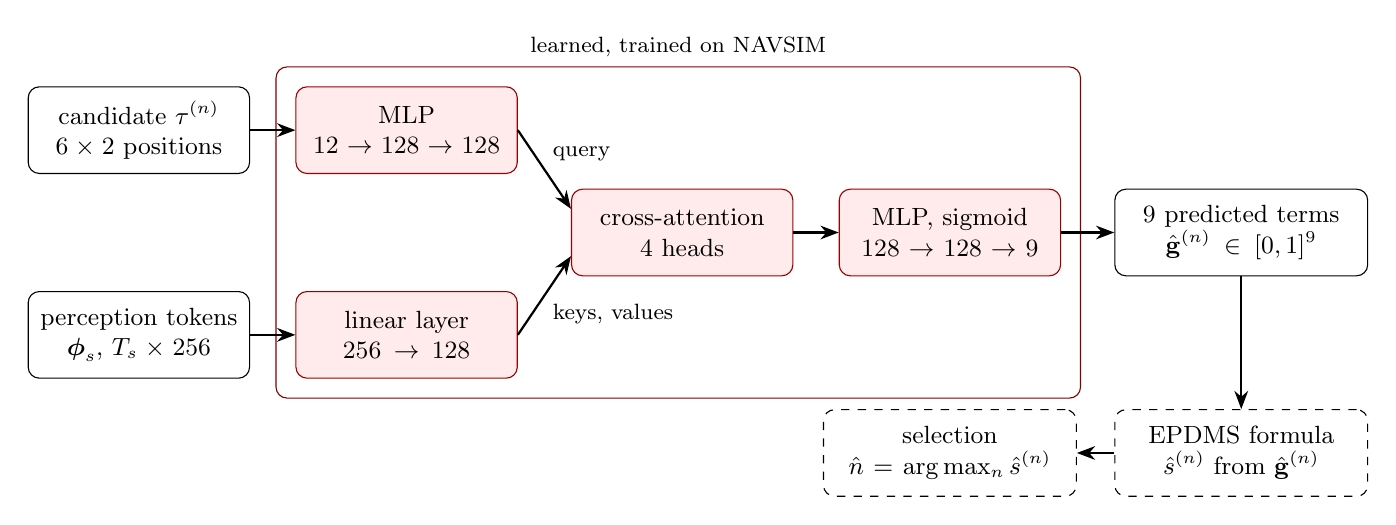
\begin{tikzpicture}[
  font=\small, >=Stealth,
  box/.style={draw,rounded corners,align=center,minimum height=1.1cm,text width=2.6cm,inner sep=3pt},
  inp/.style={box,fill=white},
  lrn/.style={box,fill=red!8,draw=red!60!black},
  fix/.style={box,fill=white,dashed,text width=3.0cm},
  flow/.style={->,thick},
]
\node[inp] (tau) at (0,1.3)  {candidate $\tau^{(n)}$\\$6\times2$ positions};
\node[inp] (phi) at (0,-1.3) {perception tokens\\$\boldsymbol\phi_s$, $T_s\times256$};
\node[lrn] (enc) at (3.4,1.3)  {MLP\\$12\to128\to128$};
\node[lrn] (prj) at (3.4,-1.3) {linear layer\\$256\to128$};
\node[lrn] (att) at (6.9,0.0)  {cross-attention\\4 heads};
\node[lrn] (hd)  at (10.3,0.0) {MLP, sigmoid\\$128\to128\to9$};
\node[inp,text width=3.0cm] (g) at (14.0,0.0) {9 predicted terms\\$\hat{\mathbf g}^{(n)}\in[0,1]^9$};
\node[fix] (rec) at (14.0,-2.8) {EPDMS formula\\$\hat s^{(n)}$ from $\hat{\mathbf g}^{(n)}$};
\node[fix] (sel) at (10.3,-2.8) {selection\\$\hat n=\arg\max_n \hat s^{(n)}$};
\draw[flow] (tau) -- (enc);
\draw[flow] (phi) -- (prj);
\draw[flow] (enc.east) -- node[above right=-1pt,font=\footnotesize]{query} ([yshift=3mm]att.west);
\draw[flow] (prj.east) -- node[below right=-1pt,font=\footnotesize]{keys, values} ([yshift=-3mm]att.west);
\draw[flow] (att) -- (hd);
\draw[flow] (hd) -- (g);
\draw[flow] (g) -- (rec);
\draw[flow] (rec) -- (sel);
\begin{scope}[on background layer]
\node[draw=red!50!black,rounded corners,fit=(enc)(prj)(att)(hd),inner sep=7pt,
      label={[font=\footnotesize]above:learned, trained on NAVSIM}] {};
\end{scope}
\end{tikzpicture}%
}
\caption[The learned scorer]{\textbf{The learned scorer.} For each candidate, an MLP encodes its six
positions into a query that attends over the perception tokens. An MLP predicts the nine EPDMS
terms from the result. The EPDMS formula combines them into one score, and the candidate with
the highest score is selected. Only the parts inside the frame are learned.}
\label{fig:scorer}
\end{figure}


\section{Inference}
\label{sec:inference}
Algorithm~\ref{alg:inference} lists the steps for one scene. The understanding and perception
experts run once; their keys and values are cached and reused by every run of the action
expert. All modes start from the same noise, so their candidates differ only through the mode
embeddings.

\begin{algorithm}[ht]
\caption{Inference for one scene}
\label{alg:inference}
\begin{algorithmic}[1]
\Require camera images and projections $P'_v$, ego history $\mathbf h$, command $c$
\State run the understanding and perception experts; cache their keys and values; keep
$\boldsymbol\phi_s$
\State draw $\boldsymbol\epsilon\sim\mathcal{N}(0,I)$, shared by all modes
\For{$n=0,\dots,N-1$}
  \State $\mathbf{x}_1\gets\boldsymbol\epsilon$
  \For{$t=1,\ 1-\delta,\ \dots,\ \delta$}
    \State $\mathbf{x}_{t-\delta}\gets\mathbf{x}_t-\delta\,v_\theta(\mathbf{x}_t,t,s,n)$
  \EndFor
  \State $\tau^{(n)}\gets$ positions from $\mathbf{x}_0$
  \State $\hat{s}^{(n)}\gets\mathrm{EPDMS}\big(g_\phi(\tau^{(n)},\boldsymbol\phi_s)\big)$
\EndFor
\State $\hat n\gets\arg\max_n\hat{s}^{(n)}$
\State \Return $\tau^{(\hat n)}$ converted to NAVSIM poses (Section~\ref{sec:output})
\end{algorithmic}
\end{algorithm}

% ============================================================================
\chapter{Experiments}
\label{ch:experiments}
% ============================================================================
This chapter describes the experiments in the order in which they were run:
\begin{enumerate}
  \item a check of the evaluation pipeline with the released UniDriveVLA
  (Section~\ref{sec:zeroshot});
  \item a test of whether the released model produces different trajectories for different
  random starting values (Section~\ref{sec:diversity});
  \item the training of the eight mode embeddings and the choice of the checkpoint
  (Section~\ref{sec:modesresult});
  \item the evaluation of the eight candidates on navhard (Section~\ref{sec:candresult});
  \item the training and evaluation of the learned scorer (Section~\ref{sec:scorerresult});
  \item an ablation of the scorer (Section~\ref{sec:ablation}).
\end{enumerate}
Sections~\ref{sec:setup} and~\ref{sec:metrics} first describe the setup and the metrics.

\section{Experimental setup}
\label{sec:setup}

\paragraph{Data.} The mode embeddings are trained on the nuScenes training split
(\num{28130} samples), and the checkpoint is selected on the nuScenes validation split
(Section~\ref{sec:modesresult}). All driving evaluations use NAVSIM v2. Its warm-up split (220 scenes) is used to
check the pipeline. All results are reported on navhard, the test split of NAVSIM v2. Navhard
contains 450 real scenes and \num{5462} synthetic second-stage scenes generated from them,
\num{5912} scenes in total. UniDriveVLA is not trained on NAVSIM v2 data.

\paragraph{Hardware.} The mode embeddings were trained on eight NVIDIA A100 GPUs with
\SI{80}{GB} each. Each GPU processes one sample per iteration, so one iteration covers eight
samples. In every iteration, the joint transformer of all three experts runs nine times: once
without a mode embedding and once per mode. An iteration took about one minute, measured in a
first run with the same setup. NAVSIM v2's scoring runs on CPUs; scoring one candidate on all
navhard scenes takes one to two hours.

\paragraph{Code.} The code, the trained mode embeddings and the instructions to reproduce all
results are available at \url{https://github.com/abdo75/unidrivevla-8-mode}.

\paragraph{Settings.} Table~\ref{tab:hparams} lists the training settings of the mode
embeddings and of the scorer. The planner outputs $N=8$ candidates per scene.

\begin{table}[ht]
\centering
\caption[Training settings]{Training settings of the mode embeddings and the scorer.}
\label{tab:hparams}
\begin{tabularx}{\linewidth}{@{}l>{\raggedright\arraybackslash}X@{}}
\toprule
Setting & Value \\
\midrule
Number of modes $N$ & 8 \\
Mode-embedding dimension $d$ & 1024 \\
Mode initialisation & Gaussian, mean 0, standard deviation 0.08 \\
Relaxed winner-takes-all share $\eta$ & 0.05 \\
Optimiser & AdamW \\
Learning rate & $1\times10^{-4}$; mode table $5\times10^{-4}$ \\
Schedule & cosine over \num{17580} iterations, 500 warm-up iterations \\
Training data & nuScenes training split (\num{28130} samples) \\
Batch & 8 GPUs $\times$ 1 sample, gradient accumulation over 4 iterations \\
Selected checkpoint & iteration \num{7000} (Section~\ref{sec:modesresult}) \\
\midrule
Scorer: optimiser & AdamW, learning rate $10^{-3}$ \\
Scorer: training & 200 epochs per cross-validation group \\
Scorer: loss & BCE $+$ ranking term, $\lambda=1$, margin $\mu=0.02$ \\
\bottomrule
\end{tabularx}
\end{table}

\paragraph{Evaluation pipeline.}
\label{sec:pipeline}
UniDriveVLA and NAVSIM's scoring code require incompatible versions of PyTorch, so they cannot
run in one Python environment. The evaluation therefore runs in three steps that only exchange
files (Figure~\ref{fig:pipeline}). The NAVSIM side writes the model inputs
(Section~\ref{sec:geometry}). The UniDriveVLA side writes the candidates and the scorer's
selection. The NAVSIM side converts the trajectories (Section~\ref{sec:output}) and scores them.

\begin{figure}[t]
\centering
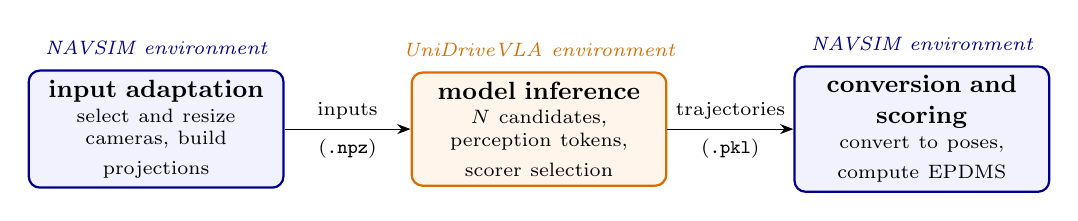
\begin{tikzpicture}[font=\small, >=Stealth,
  stg/.style={draw, rounded corners, align=center, minimum height=1.3cm, text width=3.0cm, thick},
  nav/.style={stg, draw=blue!55!black, fill=blue!5},
  uni/.style={stg, draw=orange!85!black, fill=orange!8},
  lbl/.style={font=\scriptsize}, env/.style={font=\scriptsize\itshape}
]
  \node[nav] (a) {\textbf{input adaptation}\\[1pt]\scriptsize select and resize\\\scriptsize cameras, build\\\scriptsize projections};
  \node[uni, right=1.6cm of a] (b) {\textbf{model inference}\\[1pt]\scriptsize $N$ candidates,\\\scriptsize perception tokens,\\\scriptsize scorer selection};
  \node[nav, right=1.6cm of b] (c) {\textbf{conversion and}\\\textbf{scoring}\\[1pt]\scriptsize convert to poses,\\\scriptsize compute EPDMS};
  \draw[->] (a) -- node[lbl,above]{inputs} node[lbl,below]{(\texttt{.npz})} (b);
  \draw[->] (b) -- node[lbl,above]{trajectories} node[lbl,below]{(\texttt{.pkl})} (c);
  \node[env, blue!55!black,  above=2pt of a] {NAVSIM environment};
  \node[env, orange!85!black, above=2pt of b] {UniDriveVLA environment};
  \node[env, blue!55!black,  above=2pt of c] {NAVSIM environment};
\end{tikzpicture}
\caption[Evaluation pipeline]{\textbf{Evaluation pipeline.} UniDriveVLA and NAVSIM run in separate
software environments and only exchange files.}
\label{fig:pipeline}
\end{figure}

\section{Evaluation metrics}
\label{sec:metrics}

\paragraph{EPDMS.} The main metric is EPDMS (Section~\ref{sec:epdms}), multiplied by 100. All
published NAVSIM v2 results use it.

\paragraph{Stage score.}
\label{sec:evalq}
EPDMS evaluates a planner as a whole. It is not suited to analysing the selection among
candidates, for two reasons. First, the stages are coupled: the trajectory chosen in the first
stage decides where it ends, and therefore how much each second-stage scene counts
(Section~\ref{sec:epdms}). Choosing a different candidate in one scene thus changes the score of
other scenes, and an oracle that picks the best candidate scene by scene is not defined.
Second, every EPDMS value requires a separate scoring run of NAVSIM v2
(Section~\ref{sec:setup}); we ran it for mode~0, for each single mode, and for the scorer.

To analyse the selection, we therefore also use the stage score $m(\tau,s)$ of
Equation~\eqref{eq:epdms}: the score of one trajectory $\tau$ in one scene $s$, combined from
its nine terms, before the two stages are combined into EPDMS. It is computed for each of the
\num{5912} navhard scenes, first-stage and second-stage, from that scene's trajectory alone, so
choosing a candidate in one scene affects only that scene. It is also the quantity the scorer predicts
(Section~\ref{sec:selection}). We report its mean over all scenes, multiplied by 100. Because
\num{5462} of the \num{5912} scenes are second-stage scenes, this mean is dominated by the
second stage. The stage score is used only to compare selection policies on our own
candidates. Its values differ from
EPDMS, and all comparisons with published planners use EPDMS.

For the candidates $\tau^{(n)}_s$, $n=0,\dots,N-1$, of a
scene $s$ in the set $S$ of navhard scenes, we compare five selection policies:
\begin{align}
  \mathrm{default}    &= \tfrac{1}{|S|}\textstyle\sum_{s} m\big(\tau^{(0)}_s,s\big), \\
  \mathrm{random}     &= \tfrac{1}{|S|}\textstyle\sum_{s} \tfrac{1}{N}\sum_{n} m\big(\tau^{(n)}_s,s\big), \\
  \mathrm{scorer}     &= \tfrac{1}{|S|}\textstyle\sum_{s} m\big(\tau^{(\hat n_s)}_s,s\big), \\
  \mathrm{best\text{-}fixed} &= \max_{n}\ \tfrac{1}{|S|}\textstyle\sum_{s} m\big(\tau^{(n)}_s,s\big), \\
  \mathrm{oracle}     &= \tfrac{1}{|S|}\textstyle\sum_{s} \max_{n}\ m\big(\tau^{(n)}_s,s\big).
\end{align}
The default always uses mode~0. Random is the expected score when a candidate is chosen at
random in each scene; a scorer that uses information about the scene must exceed it. The scorer
uses the candidate $\hat n_s$ selected by the learned scorer. The best fixed mode uses the same
mode in every scene, chosen with the true scores of the evaluation scenes. The oracle uses the
true score of every candidate, so it is an upper bound for any selector.

\section{Pipeline check}
\label{sec:zeroshot}
We first scored a constant-velocity agent, which ignores the cameras and keeps the current
speed, and then the released UniDriveVLA, on the warm-up split (Table~\ref{tab:prelim}). A wrong
input conversion would reduce UniDriveVLA's score to the level of the constant-velocity agent.
UniDriveVLA scores 10.4 points higher. This check used the lateral sign $\zeta=+1$, which was
corrected later (Section~\ref{sec:output}); it was not repeated with the corrected sign.

\begin{table}[ht]
\centering
\caption[Pipeline check on the warm-up split]{Pipeline check on the NAVSIM v2 warm-up split
(220 scenes).}
\label{tab:prelim}
\begin{tabular}{lc}
\toprule
Agent & EPDMS \\
\midrule
Constant velocity (ignores the cameras) & 18.5 \\
UniDriveVLA (released, single trajectory) & 28.9 \\
\bottomrule
\end{tabular}
\end{table}

\section{Diversity of the released model}
\label{sec:diversity}
On five warm-up scenes, we ran the released action expert six times per scene with different
random starting values. The endpoints of the six trajectories differed by about
\SI{0.1}{\metre} at a distance of about \SI{26}{\metre}. The released model therefore does not
provide candidates by itself, which is the reason for the mode embeddings of
Section~\ref{sec:modes}.

\section{Training the mode embeddings}
\label{sec:modesresult}
We trained the mode embeddings for \num{17580} iterations. Since each iteration covers eight
samples, this corresponds to five epochs of the nuScenes training split. To choose a checkpoint
without using NAVSIM data, we evaluated checkpoints on 500 samples of the nuScenes validation
split. For 72 of them the recorded future is shorter than \SI{3}{\second}, so 428 samples
remain. On these, we measure the minimum average displacement error over the $N$ candidates,
\begin{equation}
  \mathrm{minADE}_N=\min_{n}\ \tfrac{1}{T}\textstyle\sum_{k=1}^{T}\big\lVert\mathbf{p}^{(n)}_k-\mathbf{p}^{\star}_k\big\rVert,
\end{equation}
with recorded positions $\mathbf{p}^{\star}_k$. It measures whether \emph{some} candidate is
close to the recorded trajectory.
Figure~\ref{fig:convergence} shows that $\mathrm{minADE}_8$ falls from \SI{0.98}{\metre} after
\num{1000} iterations to \SI{0.80}{\metre} after \num{7000} and does not improve afterwards
(\SI{0.82}{\metre} after \num{17580}). We therefore use the checkpoint at iteration \num{7000},
which corresponds to two epochs and about five days of training. The error of mode~0 alone stays
between \SI{1.16}{\metre} and \SI{1.28}{\metre}.

\begin{figure}[ht]
\centering
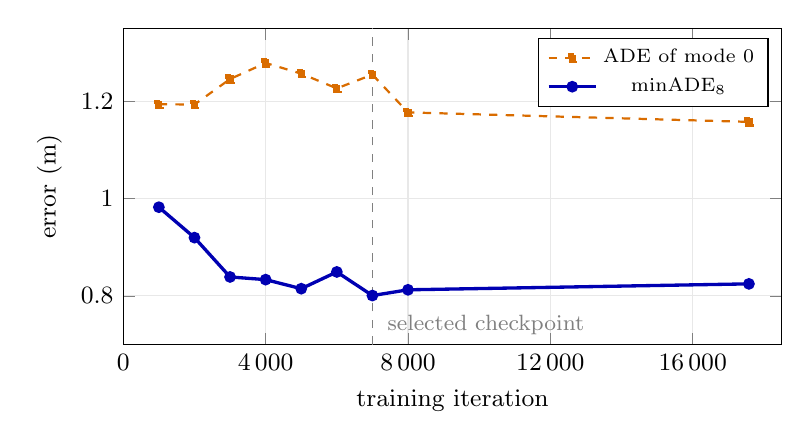
\begin{tikzpicture}
\begin{axis}[
  width=0.82\linewidth, height=5.6cm,
  xlabel={training iteration}, ylabel={error (m)},
  xmin=0, xmax=18500, ymin=0.7, ymax=1.35,
  scaled x ticks=false, xtick={0,4000,8000,12000,16000},
  xticklabel style={/pgf/number format/1000 sep={\,}},
  grid=major, grid style={gray!18},
  legend style={font=\scriptsize, at={(0.98,0.97)}, anchor=north east},
  label style={font=\small}, tick label style={font=\small},
]
\addplot[orange!85!black, thick, dashed, mark=square*, mark size=1.3pt] coordinates {
(1000,1.1938)(2000,1.1933)(3000,1.2456)(4000,1.2786)(5000,1.2567)(6000,1.2264)
(7000,1.2547)(8000,1.1771)(17580,1.1576)};
\addlegendentry{ADE of mode 0}
\addplot[blue!70!black, very thick, mark=*, mark size=1.5pt] coordinates {
(1000,0.9823)(2000,0.9198)(3000,0.8390)(4000,0.8335)(5000,0.8149)(6000,0.8493)
(7000,0.8008)(8000,0.8126)(17580,0.8248)};
\addlegendentry{$\mathrm{minADE}_8$}
\draw[gray, dashed] (axis cs:7000,0.7) -- (axis cs:7000,1.35);
\node[gray, font=\footnotesize, anchor=north west] at (axis cs:7150,0.78) {selected checkpoint};
\end{axis}
\end{tikzpicture}
\caption[Checkpoint selection for the mode training]{\textbf{Checkpoint selection for the mode
training} on 428 nuScenes validation samples. Checkpoints were evaluated every \num{1000}
iterations up to \num{8000} and at the end of training (\num{17580}).}
\label{fig:convergence}
\end{figure}

\section{Candidates on navhard}
\label{sec:candresult}
We then scored each of the eight candidates on all navhard scenes, using the same mode in every
scene (Table~\ref{tab:permode}). Mode~0 scores \num{10.0} EPDMS and mode~6, the best single
mode, \num{12.0}. In mean stage score, mode~0 reaches \num{24.4}, a random candidate \num{24.2},
and the oracle \num{34.6}, \num{10.3} points (\SI{42}{\percent}) above mode~0. In
\SI{53.1}{\percent} of the scenes all eight candidates receive the same stage score. Mode~0
scores exactly zero in \SI{63.2}{\percent} of the scenes.

\begin{table}[ht]
\centering
\caption[Scores of the eight candidates on navhard]{Scores of each of the eight candidates on
navhard when the same mode is used in every scene.}
\label{tab:permode}
\small
\setlength{\tabcolsep}{5pt}
\begin{tabular}{@{}lcccccccc@{}}
\toprule
Mode & 0 & 1 & 2 & 3 & 4 & 5 & 6 & 7 \\
\midrule
EPDMS & 10.0 & 7.9 & 9.2 & 9.3 & 9.8 & 10.5 & \textbf{12.0} & 8.7 \\
Mean stage score & 24.4 & 21.2 & 24.4 & 23.7 & 24.5 & 24.8 & \textbf{27.0} & 23.6 \\
\bottomrule
\end{tabular}
\end{table}

\section{Learned scorer}
\label{sec:scorerresult}

\paragraph{Training data.} DrivoR trains its scorer on NAVSIM's training split (navtrain) and
evaluates it on navhard. We could not do the same within our compute budget. The scorer's
training labels are the true EPDMS terms of each candidate. Producing them for navtrain would
require scoring all eight candidates of every navtrain scene, and navtrain has many times more
scenes than navhard. For navhard, these labels already exist, because computing them is part of
the evaluation in Section~\ref{sec:candresult}.

A scorer must not be evaluated on the scenes it was trained on. We therefore use five-fold
cross-validation (Figure~\ref{fig:cv}a). We split the \num{5912} navhard scenes at random into
five groups of about \num{1180} scenes and train five scorers. Each scorer is trained on four
groups and selects the candidates in the remaining group. In this way, every scene is selected
by a scorer that was not trained on it.

% Five-fold cross-validation of the scorer on navhard, and why variants of one real scene leak.
\begin{figure}[!htb]
\centering
\resizebox{\linewidth}{!}{%
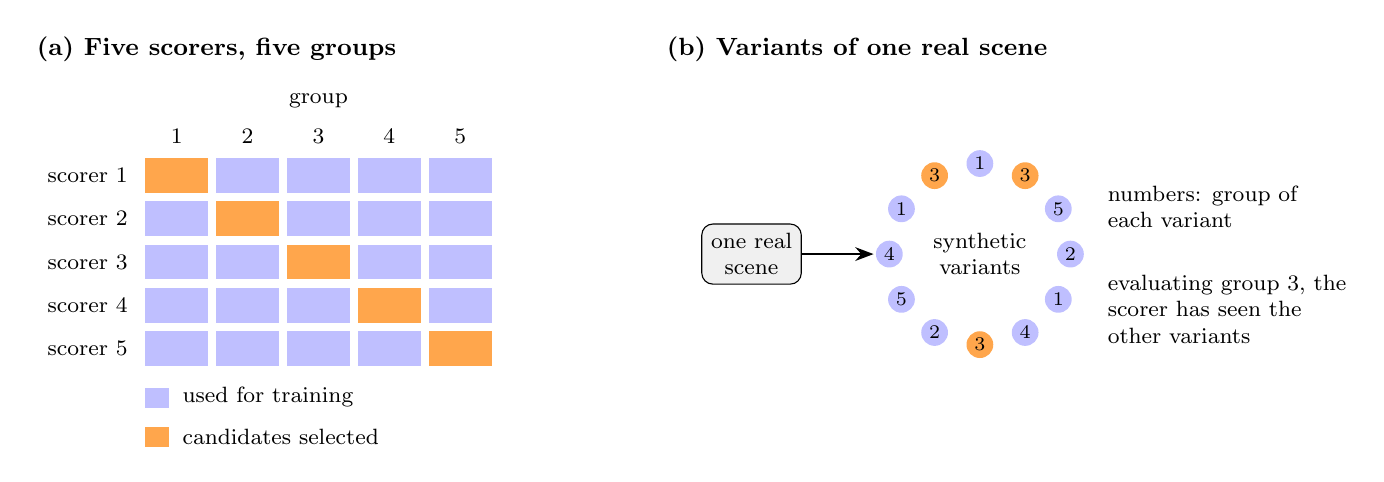
\begin{tikzpicture}[font=\footnotesize,>=Stealth]
  % ---------------- (a) folds ----------------
  \node[anchor=west,font=\small\bfseries] at (-1.0,1.6) {(a) Five scorers, five groups};
  \node at (2.7,0.95) {group};
  \foreach \c in {1,...,5} \node at (\c*0.9,0.5) {\c};
  \foreach \r in {1,...,5}{
    \node[anchor=east] at (0.4,{-(\r-1)*0.55}) {scorer \r};
    \foreach \c in {1,...,5}{
      \ifnum\r=\c
        \fill[orange!70] ({\c*0.9-0.4},{-(\r-1)*0.55-0.22}) rectangle ({\c*0.9+0.4},{-(\r-1)*0.55+0.22});
      \else
        \fill[blue!25] ({\c*0.9-0.4},{-(\r-1)*0.55-0.22}) rectangle ({\c*0.9+0.4},{-(\r-1)*0.55+0.22});
      \fi
    }
  }
  \fill[blue!25] (0.5,-2.95) rectangle (0.8,-2.7); \node[anchor=west] at (0.85,-2.82) {used for training};
  \fill[orange!70] (0.5,-3.45) rectangle (0.8,-3.2); \node[anchor=west] at (0.85,-3.32) {candidates selected};
  % ---------------- (b) leakage ----------------
  \begin{scope}[xshift=7.6cm]
    \node[anchor=west,font=\small\bfseries] at (-0.6,1.6) {(b) Variants of one real scene};
    \node[draw,rounded corners,fill=gray!12,align=center] (r) at (0.6,-1.0) {one real\\scene};
    \foreach \i/\g [count=\k] in {1/1,2/3,3/5,4/2,5/1,6/4,7/3,8/2,9/5,10/4,11/1,12/3}{
      \pgfmathsetmacro\ang{90-(\k-1)*30}
      \ifnum\g=3
        \fill[orange!70] ($(3.5,-1.0)+(\ang:1.15)$) circle (0.17);
      \else
        \fill[blue!25] ($(3.5,-1.0)+(\ang:1.15)$) circle (0.17);
      \fi
      \node[font=\scriptsize] at ($(3.5,-1.0)+(\ang:1.15)$) {\g};
    }
    \draw[->,thick] (r.east) -- (2.15,-1.0);
    \node[align=center] at (3.5,-1.0) {synthetic\\variants};
    \node[align=left,anchor=west] at (5.0,-0.4) {numbers: group of\\each variant};
    \node[align=left,anchor=west] at (5.0,-1.7) {evaluating group 3, the\\scorer has seen the\\other variants};
  \end{scope}
\end{tikzpicture}%
}
\caption[Cross-validation of the scorer on navhard]{\textbf{Cross-validation of the scorer on
navhard.} (a) Each of five scorers is trained on four groups and selects the candidates in the
remaining group. (b) The groups are formed at random over all scenes, so the synthetic variants
of one real scene fall into different groups.}
\label{fig:cv}
\end{figure}


\paragraph{Limits of this evaluation.} Each of the 450 real scenes of navhard has about twelve
synthetic variants, which show the same road and traffic from slightly shifted positions of the
ego vehicle. Because the groups are formed at random over all scenes, the variants of one real
scene end up in different groups (Figure~\ref{fig:cv}b). A scorer that selects a candidate in
one variant may therefore have been trained on other variants of the same real scene. This makes
its task easier than on a scene it has never seen, so the result may be higher than on new
scenes. Forming the groups by real scene would avoid this. In addition, NAVSIM v2 does not allow
training on navhard for leaderboard entries, so our result with the scorer cannot be submitted
as one.

\paragraph{Results.} Table~\ref{tab:selection} compares the five selection policies in mean stage
score. The scorer reaches \num{26.8}, against \num{24.4} for mode~0 and \num{24.2} for a random
candidate. It recovers \SI{24}{\percent} of the distance from mode~0 to the oracle. It is
\num{0.2} points below the best fixed mode, which is chosen with the true scores. Per scene, the
scorer selects a better candidate than mode~0 in \SI{29.0}{\percent} of the scenes, an equally
scored one in \SI{61.8}{\percent}, and a worse one in \SI{9.3}{\percent}. Figure~\ref{fig:selhist}
shows how often it selects each mode: mode~6, the best single mode, in \SI{46.5}{\percent} of the
scenes, and mode~1, the weakest single mode in EPDMS (\num{7.9}), in \SI{20.1}{\percent}.

\begin{table}[ht]
\centering
\caption[Selection policies on navhard]{Selection policies on navhard, mean stage score.}
\label{tab:selection}
\begin{tabular}{lc}
\toprule
Policy (over 8 candidates) & mean stage score \\
\midrule
Default (mode 0)                      & 24.4 \\
Random candidate                      & 24.2 \\
Learned scorer                        & 26.8 \\
Best fixed mode in hindsight (mode 6) & 27.0 \\
Oracle (best of 8 per scene)          & \textbf{34.6} \\
\bottomrule
\end{tabular}
\end{table}

\begin{figure}[ht]
\centering
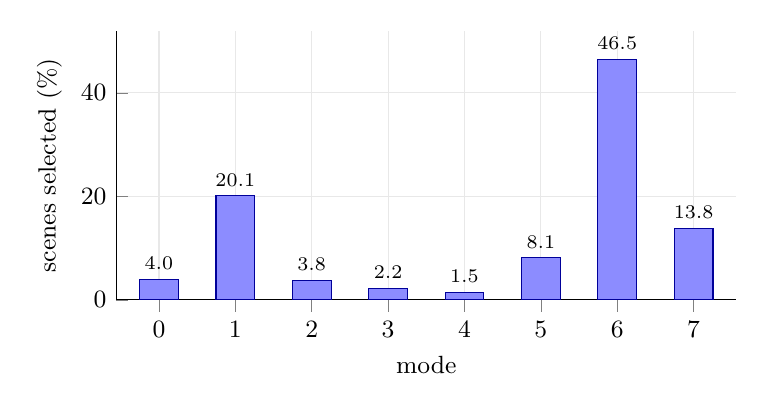
\begin{tikzpicture}
\begin{axis}[
  width=0.78\linewidth, height=5.0cm,
  ybar, bar width=14pt, ymin=0, ymax=52,
  ylabel={scenes selected (\%)}, xlabel={mode},
  symbolic x coords={0,1,2,3,4,5,6,7}, xtick=data,
  nodes near coords={\pgfmathprintnumber[fixed,fixed zerofill,precision=1]{\pgfplotspointmeta}},
  every node near coord/.append style={font=\scriptsize},
  label style={font=\small}, tick label style={font=\small},
  grid=major, grid style={gray!18}, enlarge x limits=0.08, axis x line*=bottom, axis y line*=left,
]
\addplot[fill=blue!45, draw=blue!60!black] coordinates {
(0,4.0)(1,20.1)(2,3.8)(3,2.2)(4,1.5)(5,8.1)(6,46.5)(7,13.8)};
\end{axis}
\end{tikzpicture}
\caption[Modes selected by the learned scorer]{\textbf{Modes selected by the learned scorer}
in the \num{5912} navhard scenes.}
\label{fig:selhist}
\end{figure}

\paragraph{Comparison with published planners.}
\label{sec:navhard}
Table~\ref{tab:navhard} compares the planner with published planners in EPDMS. To our
knowledge, UniDriveVLA has not been evaluated on NAVSIM before; its authors report results on
nuScenes and in closed-loop simulation. To our knowledge, SparseDrive and VAD have no published
navhard results, so they are not listed. Our pipeline scores the constant-velocity agent at
\num{11.5}, close to the published \num{10.9}. The released UniDriveVLA was not scored on navhard
with the corrected lateral sign, so the table contains no result of the released model; mode~0
of the eight-mode model is the single-trajectory reference. With the scorer, the planner scores \num{12.7},
\SI{27}{\percent} more than mode~0 (\num{10.0}) and \num{0.7} points more than the best fixed mode
(\num{12.0}). It equals the ego-status MLP (\num{12.7}), scores above the constant-velocity
agent, and scores below Latent TransFuser (\num{23.1}), the candidate-selection planners GTRS
(\num{45.0}), ZTRS (\num{48.1}), and DrivoR (\num{48.3}), and PDM-Closed (\num{51.3}).

\begin{table}[ht]
\centering
\caption[EPDMS on navhard]{EPDMS (higher is better) on navhard. The reference
planners are trained on NAVSIM; values from \cite{pseudosim} and from Table~3 of
\cite{drivor}. UniDriveVLA
is not trained on NAVSIM; the learned scorer is trained on navhard with five-fold
cross-validation.}
\label{tab:navhard}
\begin{tabular}{lc}
\toprule
Method & EPDMS $\uparrow$ \\
\midrule
Constant velocity \cite{pseudosim} & 10.9 \\
Ego-status MLP \cite{pseudosim} & 12.7 \\
Latent TransFuser \cite{transfuser,pseudosim} & 23.1 \\
GTRS-D \cite{gtrs,drivor} & 45.0 \\
ZTRS \cite{ztrs,drivor} & 48.1 \\
DrivoR \cite{drivor} & 48.3 \\
PDM-Closed \cite{pdm} & 51.3 \\
\midrule
UniDriveVLA, eight modes, mode~0 & 10.0 \\
UniDriveVLA, eight modes, best fixed mode in hindsight & 12.0 \\
\textbf{UniDriveVLA, eight modes + learned scorer} & \textbf{12.7} \\
\bottomrule
\end{tabular}
\end{table}

\section{Ablation of the scorer}
\label{sec:ablation}

\begin{table}[ht]
\centering
\caption[Ablation of the scorer on navhard]{Ablation of the scorer on navhard (mean stage
score). Mode~0 is replaced only when the predicted gain exceeds $\tau$; $\tau=0$ is the plain
$\arg\max$, and $\tau=\infty$ removes the scorer.}
\label{tab:ablscorer}
\begin{tabular}{lcccccc}
\toprule
Margin $\tau$ & 0 & 1 & 2 & 5 & 10 & $\infty$ (always mode 0) \\
\midrule
Mean stage score & \textbf{26.8} & 26.2 & 26.2 & 26.1 & 25.6 & 24.4 \\
\bottomrule
\end{tabular}
\end{table}

Finally, we reduced the influence of the scorer step by step. Mode~0 is replaced by the
scorer's choice only when the predicted score of that choice exceeds the predicted score of
mode~0 by more than a margin $\tau$ (in points). With $\tau=\infty$, the scorer is removed and
mode~0 is always used. Table~\ref{tab:ablscorer} shows that the mean stage score decreases from
\num{26.8} at $\tau=0$ to \num{24.4} at $\tau=\infty$. This ablation uses the evaluation scenes,
so it was not used to choose $\tau$; the reported scorer uses $\tau=0$, fixed in advance. The
other ablations listed in Section~\ref{sec:limits} could not be run.

% ============================================================================
\chapter{Discussion}
\label{ch:discussion}
% ============================================================================
This chapter interprets the results of Chapter~\ref{ch:experiments}, shows examples of
individual scenes, and discusses the limitations of this work and possible next steps.

\section{Interpretation of the results}
\label{sec:interpretation}

\paragraph{Why the scorer improves the planner.} The eight candidates of a scene differ in ways
that EPDMS rewards: an oracle that picks the best candidate in each scene reaches a mean stage
score of \num{34.6}, against \num{24.4} for mode~0. The scorer recovers about a quarter of this
difference. It is above a random choice of candidate (\num{24.2}), so its predicted ranking carries
information about which candidate scores higher. Its choice depends on the scene: it selects mode~6,
the best single mode, in about half of the scenes, but it also selects mode~1, the weakest mode
when used in every scene, in a fifth of the scenes. A fixed choice of mode cannot vary in this
way. Compared with mode~0, the scorer's choice is better three times as often as it is worse
(\SI{29.0}{\percent} against \SI{9.3}{\percent} of the scenes). This is consistent with the
ablation in Section~\ref{sec:ablation}: every margin that limits how often the scorer may
replace mode~0 lowers the result.

\paragraph{Why mode~0 is a weak default.} Relaxed winner-takes-all training updates mainly the
mode that is closest to the recorded trajectory in each scene. The modes therefore specialise on
different scenes, and no mode, including mode~0, is trained to be good in every scene. The
training curve shows this: $\mathrm{minADE}_8$ improves while the error of mode~0 alone does
not (Figure~\ref{fig:convergence}). The scorer selects mode~0 in only \SI{4.0}{\percent} of the
scenes.

\paragraph{Why the absolute score is low.} Mode~0 scores exactly zero in \SI{63.2}{\percent} of
the navhard scenes. A zero requires at least one penalty term to be zero: an at-fault
collision, leaving the drivable area, driving against the lane direction, or passing a red
light. In \SI{53.1}{\percent} of the scenes all eight candidates receive the same stage score,
so no selector can improve these scenes. Most of the gap to the strongest planners therefore
most likely comes from the candidates themselves, not from the selection. Table~\ref{tab:design} compares
the planners on the design choices that differ.

\begin{table}[ht]
\centering
\caption[Design of the compared planners]{Design of the compared planners. ``Training data'' is
the data the planner is trained on; ``Backbone'' states how the image encoder is adapted to
NAVSIM; ``Cand.'' is the number of candidate trajectories per scene. PDM-Closed reads the map
and the positions of other road users from the dataset annotations; the learned planners use
only sensors. Values for DrivoR, ZTRS, and GTRS-D from Table~3 of \cite{drivor}, the
others from \cite{pseudosim,navsim}.}
\label{tab:design}
\small
\setlength{\tabcolsep}{4pt}
\begin{tabular}{@{}>{\raggedright\arraybackslash}p{3.6cm} p{1.9cm} p{1.9cm} l c c@{}}
\toprule
Method & Inputs & Training data & Backbone & Cand. & EPDMS \\
\midrule
PDM-Closed \cite{pdm} & map, tracks & rule-based & --- & many & 51.3 \\
DrivoR \cite{drivor} & 4 cameras & navtrain & ViT-S (LoRA) & 64 & 48.3 \\
ZTRS \cite{ztrs} & cameras & navtrain & V2-99 (trained) & many & 48.1 \\
GTRS-D \cite{gtrs} & cameras & navtrain & V2-99 (trained) & many & 45.0 \\
Latent TransFuser \cite{transfuser,pseudosim} & cameras & navtrain & trained & 1 & 23.1 \\
Ego-status MLP \cite{pseudosim} & ego only & navtrain & --- & 1 & 12.7 \\
\midrule
UniDriveVLA + scorer (ours) & 6 cameras & nuScenes & frozen & 8 & 12.7 \\
\bottomrule
\end{tabular}
\end{table}

Three differences are the most likely reasons for the gap to DrivoR. First, UniDriveVLA is trained only on nuScenes,
whereas navhard is recorded with other vehicles and cameras and partly in other cities; DrivoR
is trained on navtrain. Second, UniDriveVLA's backbone is frozen: we train about \num{5.3}
million of its roughly \num{2.7} billion parameters (under \SI{0.2}{\percent}), so the
perception and understanding experts cannot adapt to NAVSIM's roads, whereas DrivoR adapts its
image encoder. Third, our candidates often receive the same score. DrivoR's own experiments show that
more candidates help when the planner is trained on the target data, with the gain levelling off
at about 64 candidates \cite{drivor}. With a frozen backbone trained elsewhere, additional modes
would likely receive the same score in the same scenes. DrivoR reaches a drivable-area compliance of \num{88.4} in
the second stage \cite{drivor}, so most of its trajectories stay on the road. In the case studies of
Section~\ref{sec:cases}, mode~0 leaves the drivable area at turns. The lateral sign of the
conversion was verified on navhard (Section~\ref{sec:output}). The most likely cause is the
domain gap: the perception expert places the trajectories using road geometry learned on
nuScenes. Two further factors may contribute. First, the model predicts \SI{3}{\second}, and
the fourth second is added by repeating the last step (Section~\ref{sec:output}). In a turn,
this extension continues straight and can leave the drivable area. Second, the second-stage
scenes, which make up most of navhard, consist of synthetic camera images, which differ from
the real images the model was trained on. Neither effect was measured separately. The mode
training converged on nuScenes (Figure~\ref{fig:convergence}); whether more training would
change the result on NAVSIM v2 was not tested.

PDM-Closed is a different case. It reads the map and the tracks of other road users from the
dataset annotations and scores its candidates with the same rules that EPDMS is built on. A
planner that uses only cameras is not expected to match it.

\section{Case studies}
\label{sec:cases}
Figure~\ref{fig:cases} shows three navhard scenes in which mode~0 leaves the drivable area
(drivable-area compliance of zero) while another candidate stays on it. The scenes were chosen
from the first-stage scenes by this criterion. In all three, the human driver turns at an
intersection. The eight candidates lie close to each other, cover a shorter distance than the
recorded trajectory, and turn less sharply. In each scene another candidate stays on the
drivable area, so a selector can avoid leaving it, but none of the candidates follows the turn
of the human driver. Part of this may come from the straight extension of the fourth second
(Section~\ref{sec:output}).

\begin{figure}[ht]
\centering
\begin{minipage}{0.31\linewidth}\centering
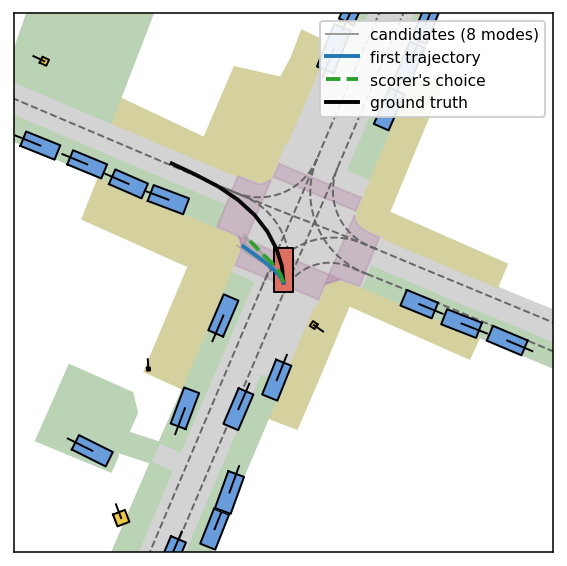
\includegraphics[width=\linewidth]{figures/cases/003_131ab0263b07507c.png}\\(a)
\end{minipage}\hfill
\begin{minipage}{0.31\linewidth}\centering
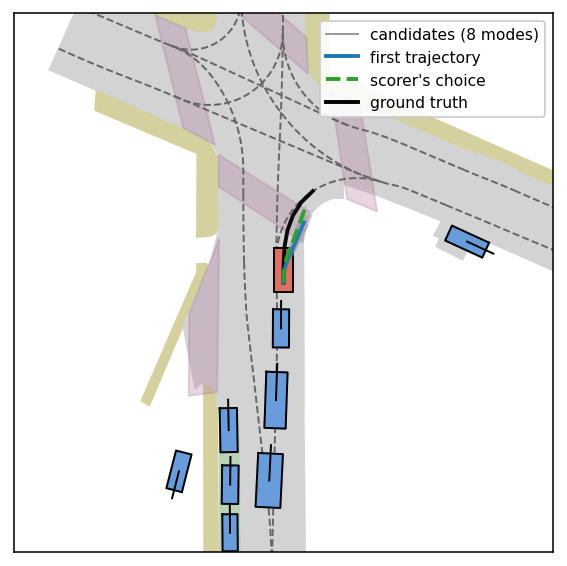
\includegraphics[width=\linewidth]{figures/cases/006_0ec9a79351355022.png}\\(b)
\end{minipage}\hfill
\begin{minipage}{0.31\linewidth}\centering
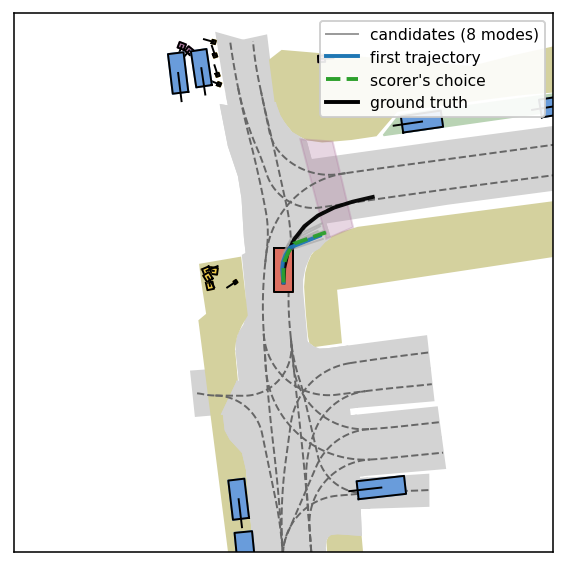
\includegraphics[width=\linewidth]{figures/cases/011_6e2c6027edb85763.png}\\(c)
\end{minipage}
\caption[Case studies on navhard]{\textbf{Case studies on navhard.} Three scenes in which mode~0
leaves the drivable area while another candidate stays on it. Grey: the eight candidates; blue
(``first trajectory''): mode~0; green, dashed: the scorer's choice; black (``ground truth''):
the recorded trajectory of the human driver; red box: ego vehicle. (a) Left turn at an intersection. (b) Right turn into a crossing road.
(c) Right turn at a junction.}
\label{fig:cases}
\end{figure}

\section{Limitations}
\label{sec:limits}
\begin{itemize}
  \item \emph{Domain and frozen backbone.} UniDriveVLA is trained only on nuScenes and its
  backbone stays frozen, so the quality of the candidates on NAVSIM v2 is limited by how well the
  model transfers. The second-stage scenes add synthetic camera images.
  \item \emph{Horizon extension.} The fourth second of every trajectory is a straight
  continuation of the last predicted step, added only for compatibility with NAVSIM v2. Its
  effect on EPDMS was not measured.
  \item \emph{No navhard result for the released model.} The released UniDriveVLA was evaluated
  only on the warm-up split, with the uncorrected lateral sign. The comparison with it on navhard
  is therefore missing.
  \item \emph{Scorer evaluation.} The cross-validation on navhard may be optimistic, and the
  result cannot be submitted to the leaderboard (Section~\ref{sec:scorerresult}).
  \item \emph{Stage score and oracle.} With more compute, EPDMS could also be computed for the
  oracle's and a random selection, by scoring each selection in a separate NAVSIM v2 run. We
  report these policies only in mean stage score, which is dominated by second-stage scenes and
  cannot be compared with published results.
  \item \emph{Missing ablations.} The number of modes, the relaxed winner-takes-all share, and
  the mode initialisation were fixed, because each setting requires a new multi-day training
  run. For the same reason, the mode embeddings were not compared in EPDMS with candidates from
  different random starting values, which Section~\ref{sec:diversity} shows to be almost
  identical. A per-term breakdown of EPDMS is not available, so the attribution of zero scores
  to specific penalty terms rests on the case studies.
  \item \emph{Ego state.} At inference the model uses its own estimate of the ego vehicle's
  motion state. Using the ego state recorded by NAVSIM v2 instead was not tested.
  \item \emph{Single run.} The mode embeddings were trained once, and the cross-validation used
  one random split. The variance of the results is unknown.
  \item \emph{Computational cost.} At inference, the action expert runs $N=8$ times with $K=10$
  steps each, while the understanding and perception experts run once. During training, the
  joint transformer runs $N+1=9$ times per iteration.
  \item \emph{Evaluation protocol.} NAVSIM v2 scores each trajectory once and does not feed it
  back to the planner, so the planner is not tested in closed loop.
\end{itemize}

\section{Future work}
\label{sec:future}
\begin{itemize}
  \item \emph{Training on NAVSIM.} Training the action expert and the mode embeddings, and in a
  second step the perception expert, on navtrain would address the domain gap and give the
  scorer candidates that stay on the road.
  \item \emph{Scorer evaluation.} Training the scorer on navtrain, or forming the
  cross-validation groups by real scene, would remove the optimism of the current evaluation and
  allow a leaderboard submission.
  \item \emph{A stronger default.} Adding the trajectory of the released planner as an
  additional candidate would give the scorer a default that is not specialised by
  winner-takes-all training.
  \item \emph{Missing analyses.} EPDMS for the released model and for the oracle's selection
  on navhard, a per-term breakdown of EPDMS, several training runs, and a comparison of
  different numbers of modes would complete the evaluation.
  \item \emph{Full horizon.} Training the action expert to predict the full \SI{4}{\second}
  of NAVSIM v2 would remove the straight extension of the last second.
  \item \emph{Closed-loop evaluation.} Testing the planner in a closed-loop simulator would show
  whether the selection also helps when errors accumulate.
\end{itemize}

\section{Conclusion}
\label{sec:conclusion}
This thesis tested whether DrivoR's approach of generating several candidate trajectories and
selecting one with a learned scorer improves the vision--language--action model UniDriveVLA,
and whether the combination reaches state-of-the-art results, without training UniDriveVLA on
NAVSIM data. We built a pipeline that evaluates
UniDriveVLA with EPDMS on NAVSIM v2. We added eight mode embeddings to the action expert and
trained them with relaxed winner-takes-all, so that the model produces eight different
candidates. A learned scorer predicts the EPDMS terms of each candidate and selects one. On
navhard, the scorer raises EPDMS from \num{10.0} for mode~0 to \num{12.7}, above every single
mode. In our cross-validated evaluation, candidate selection therefore improves the default
mode of a vision--language--action model trained on another dataset. It does not reach
state-of-the-art results: the planner scores below planners trained on NAVSIM, such as DrivoR
(\num{48.3}), most likely because many candidates violate a penalty term such as the drivable
area. Adapting the model to the target data is the main remaining step.

%% End main parts --------------------------------------------------------------
\backmatter

\bibliographystyle{unsrt}
\bibliography{references}

\end{document}
